\documentclass{article}


% if you need to pass options to natbib, use, e.g.:
% \PassOptionsToPackage{numbers, compress}{natbib}
% \PassOptionsToPackage{numbers,square,comma,sort}{natbib}

% before loading neurips_2025


% ready for submission
% \usepackage[preprint]{neurips_2025}
\usepackage[nonatbib,preprint]{neurips_2025}

% to compile a preprint version, e.g., for submission to arXiv, add add the
% [preprint] option:
%     \usepackage[preprint]{neurips_2025}


% to compile a camera-ready version, add the [final] option, e.g.:
%     \usepackage[final]{neurips_2025}


% to avoid loading the natbib package, add option nonatbib:
%    \usepackage[nonatbib]{neurips_2025}


\usepackage[utf8]{inputenc} % allow utf-8 input
\usepackage[T1]{fontenc}    % use 8-bit T1 fonts
\usepackage{hyperref}       % hyperlinks
\usepackage{url}            % simple URL typesetting
\usepackage{bm}
\usepackage{booktabs}       % professional-quality tables
\usepackage{amsfonts}       % blackboard math symbols
\usepackage{nicefrac}       % compact symbols for 1/2, etc.
\usepackage{microtype}      % microtypography
\usepackage{xcolor}         % colors
\usepackage{multirow}
\usepackage{subcaption}
\usepackage{graphicx}
\usepackage{amsmath}
\usepackage{cleveref}
\usepackage{tcolorbox}
\usepackage{colortbl}
\usepackage{array}
\usepackage{wrapfig}


% ——— BibLaTeX setup ———
\usepackage[backend=biber,
            style=numeric,
            sorting=nyt,         % “name–year–title” 
            maxbibnames=99,
            natbib=true,
            doi=false,
            isbn=false,
            url=false,
            eprint=true]{biblatex}

\DeclareFieldFormat
  [article,inbook,incollection,inproceedings,patent,thesis,
   techreport,unpublished,misc,book]
  {title}{\mkbibquote{#1}}

% format arXiv entries as “arXiv:XXXX.XXXXX”
% \DeclareFieldFormat{eprint:arxiv}{%
%   \iffieldundef{eprinttitle}
%     {\mkbibacro{arXiv}\addcolon\space
%      \ifhyperref
%        {\href{https://arxiv.org/abs/#1}{#1}}
%        {#1}}
%     {\mkbibacro{arXiv}\addcolon\space
%      \ifhyperref
%        {\href{https://arxiv.org/abs/\strfield{eprint}}{%
%          \printfield[eprinttitle]{eprint}}}
%        {\printfield[eprinttitle]{eprint}}}}

% \renewbibmacro*{eprint:arxiv+pubstate}{%
%   \usebibmacro{eprint:arxiv}}

% point at your .bib file
\addbibresource{main.bib}


% \definecolor{Gray}{gray}{0.85}
% \definecolor{LightCyan}{rgb}{0.88,1,1}

% \newcolumntype{a}{>{\columncolor{Gray}}r}
% \newcolumntype{b}{>{\columncolor{LightCyan}}r}

% define a callout style once in your preamble
\newtcolorbox{callout}{
  colback=blue!5,      % background color
  colframe=blue!40,    % border color
  left=3pt, right=3pt, top=3pt, bottom=3pt,
  boxrule=0.5pt,
  arc=2pt
}

\newcommand{\rj}[1]{\textcolor{red}{rishi:\ #1}}
\newcommand{\vs}[1]{\textcolor{purple}{vitaly:\ #1}}
\newcommand{\jm}[1]{\textcolor{orange}{jack:\ #1}}
\newcommand{\atk}{\texttt{vec2vec}}
\renewcommand{\L}{\mathcal{L}}
\newcommand{\R}{\mathbb{R}}

\newcommand{\shortpara}[1]{\vspace{.75ex}\noindent\textbf{#1}}



% \title{All Embeddings Learn (Almost) The Same Thing}
% \title{Embedding Translations with Vectors Only}
% \title{Embedding Translation from Only A Few Vectors}
% \title{Adversarial Unsupervised Embedding Alignment}
% \title{Translating Representations from Representations Alone}
% \title{Translating the Universal Language of\\ Text Embeddings}
% \title{Translating the Universal Language of Embeddings}
\title{Harnessing the Universal Geometry of Embeddings}


% The \author macro works with any number of authors. There are two commands
% used to separate the names and addresses of multiple authors: \And and \AND.
%
% Using \And between authors leaves it to LaTeX to determine where to break the
% lines. Using \AND forces a line break at that point. So, if LaTeX puts 3 of 4
% authors names on the first line, and the last on the second line, try using
% \AND instead of \And before the third author name.


\author{%
  Rishi Jha \quad Collin Zhang \quad Vitaly Shmatikov \quad John X. Morris\\
  Department of Computer Science\\
  Cornell University
  % \texttt{\{rjha01, jhayase, sewoong\}@cs.washington.edu} \\
}

\begin{document}

\maketitle

\begin{abstract}
We introduce the first method for translating text embeddings from one vector space to another without any paired data, encoders, or predefined sets of matches.  Our unsupervised approach translates any embedding to and from a universal latent representation (i.e., a universal semantic structure conjectured by the Platonic Representation Hypothesis).  Our translations achieve high cosine similarity across model pairs with different architectures, parameter counts, and training datasets.

The ability to translate unknown embeddings into a different space while preserving their geometry has serious implications for the security of vector databases.  An adversary with access only to embedding vectors can extract sensitive information about the underlying documents, sufficient for classification and attribute inference.

\end{abstract}

\begin{figure}[h]
    \centering
    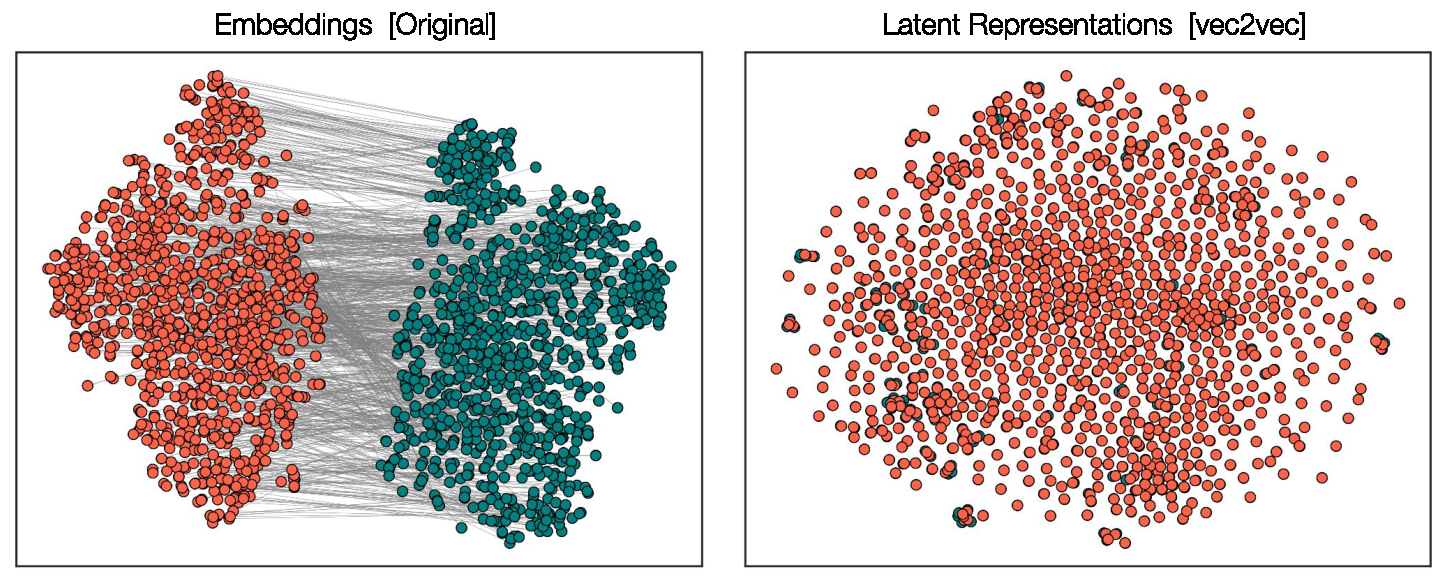
\includegraphics[width=0.8\linewidth]{ims/universal2.pdf}
    \caption{Left: input embeddings from different model families (T5-based GTR \citep{ni2021gtr} and BERT-based GTE \citep{li2023gte}) are fundamentally incomparable. Right:
    given unpaired embedding samples from different models on different texts, our model learns a latent representation where they are closely aligned.}
    \label{fig:main}
\end{figure}


\begin{figure}[t]
    \centering
    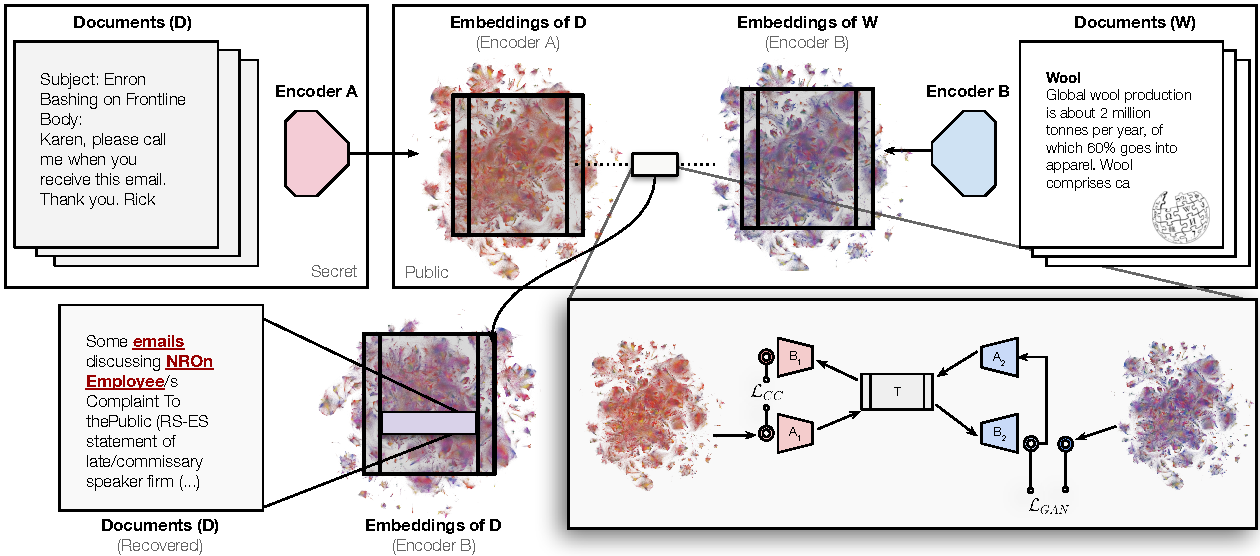
\includegraphics[width=0.85\linewidth]{ims/diagram.pdf}
    \caption{Given only a vector database from an unknown model, \atk{} translates the database into the space of a known model using latent structure alone. Converted embeddings reveal sensitive information about the original documents, such as the topic of an email (pictured, real example).}
    % https://docs.google.com/drawings/d/15lO_xIOkSc-jI75ThhHp4K_mFUQFW0nI--rZyht2avg/edit?usp=sharing
    \label{fig:architecture}
\end{figure}
\section{Introduction}

Text embeddings are the backbone of modern NLP, powering tasks like retrieval, RAG, classification, and clustering.  There are many embedding models trained on different datasets, data shufflings, and initializations.  An embedding of a text encodes its semantics: a good model maps texts with similar semantics to vectors close to each other in the embedding space.    Since semantics is a property of text, different embeddings of the same text should encode the same semantics.  In practice, however, different models encode texts into completely different and incompatible vector spaces.

% Semantics is a property of input text, and should be invariant to the embedding model chosen. However, many neural embedding models exist. These models are trained on different datasets, data shufflings, and initializations. This inconsistency has produced a world of embedding models trained on similar or identical datasets encoding the same semantics in completely different and incompatible spaces \Cref{fig:main}.

% Prior work  \citep{huh2024platonicrepresentationhypothesis} has proposed that models trained on the same modality share inevitable similarities due to their shared underlying reality (i.e. the world we live in). Another line of research develops systems to quantify this similarity between representation spaces \citep{maiorca2024latentspacetranslationsemantic, moschella2023relativerepresentationsenablezeroshot, moayeri2023texttoconceptandbackcrossmodel, norelli2023asifcoupleddataturns}. These works have achieved remarkable results including zero-shot stitching, substitution, and multi-modal adaptation without training. However, all of these methods rely on at least a small amount of paired data between the two modalities of interest; efforts to reduce the number of pairs required have proven difficult \citep{cannistraci2023bootstrappingparallelanchorsrelative}.

% \rj{The jump between these two paragraphs feels a little abrupt. Also we should converge on a wording of the hypothesis. I think we should avoid the word 'mapping'}

The Platonic Representation Hypothesis \citep{huh2024platonicrepresentationhypothesis} conjectures that all image models of sufficient size have the same latent representation.  We propose a stronger, constructive version of this hypothesis for text models: the universal latent structure of text representations can be learned and, furthermore, harnessed to translate representations from one space to another without any paired data or encoders.

In this work, we show that the Strong Platonic Representation Hypothesis holds in practice.  Given unpaired examples of embeddings from two models with different architectures and training data, our method learns a latent representation in which the embeddings are almost identical (\Cref{fig:main}).

We draw inspiration from research on aligning word embeddings across languages \citep{xing2015normalized, conneau2018wordtranslationparalleldata, grave2018unsupervisedalignmentembeddingswasserstein, chen2018unsupervisedmultilingualwordembeddings} and unsupervised image translation
\citep{liu2018unsupervisedimagetoimagetranslationnetworks,zhu2020unpairedimagetoimagetranslationusing}. Our \atk{} method uses adversarial losses and cycle consistency to learn to encode embeddings into a shared latent space and decode with minimal loss.  This makes unsupervised translation possible.  We use a basic adversarial approach with vector space preservation \citep{mrksic2016counterfittingwordvectorslinguistic} to learn a mapping from an unknown embedding distribution to a known one.

% Trained on as few as 50K unpaired samples from each model, 
\atk{} is the
\textbf{first method to successfully translate embeddings from the space of one model to another without any paired data.}
\atk{}
translations achieve cosine similarity as high as $0.92$ to the ground-truth vectors in their target embedding spaces and perfect matching on over $8000$ shuffled embeddings (without access to the set of possible matches in advance). 

To show that our translations preserve not only the relative geometry of embeddings but also the semantics of underlying inputs, we extract information from them using zero-shot attribute inference and inversion, without any knowledge of the model that produced the original embeddings!

% In one case, we are able to take a database of 100K vectors from an unknown embedding model and learn an unsupervised mapping to a known embedding space. Given our translated embeddings are then able to perform attribute extraction as well as inversion without any paired data, without making any function calls to the unknown encoder, and crucially \textit{without knowing anything about the model used to produce the embeddings}. \rj{1M (although I think the ablations will show this is true for 100K and maybe 50K).} \rj{Also confused by what the first sentence is adding--statement on data amount? Why is it "in once case"--don't we do that for all? Second sentence seems incomplete?}

% To demonstrate that our translation not only preserves relative geometry of embedding vectors (measured via cosine similarity) but also semantics, we carry out several experiments to demonstrate that we can use translation to extract essential semantic information about the text encoded in the source embeddings. We are able to perform classification on tweet embeddings and extract sensitive information from emails.


\section{Problem formulation: unsupervised embedding translation}

Consider a collection of embedding vectors $\{u_1, \ldots u_n\}$, for example, a dump of a compromised vector database, where each $u_i = M_1(d_i)$ is generated by an unknown encoder $M_1 : \mathbb{V}^s \rightarrow \R^{d_{M_1}}$ from an unknown document $d_i$.  We cannot make queries to $M_1$ and do not know its training data, nor architectural details.  Our goal is to extract any information about the documents $d_i$.

% The only available information is the cosine similarities between vectors, i.e., the embedding geometry.  


\begin{figure}[t]
    \centering
    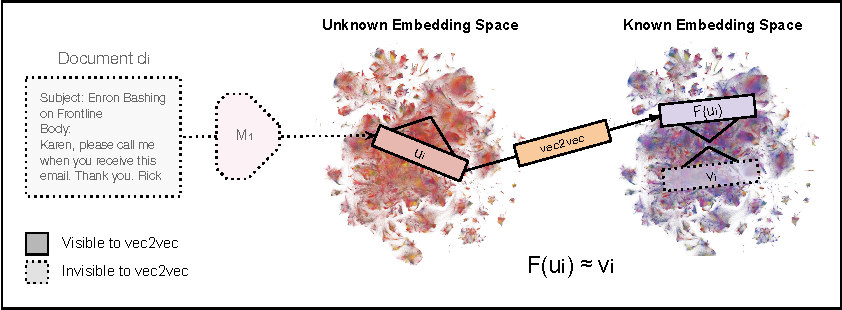
\includegraphics[width=0.9\linewidth]{ims/spaces.pdf}
    \caption{\textbf{Unsupervised embedding translation}. With access to only $u_i = M_1(d_i)$, \atk{} seeks to generate a translation $F(u_i)$ that is close in $M_2$'s embedding space to the ideal embedding $v_i = M_2(d_i)$ without access to $d_i$, $v_i$, $M_1$, or $M_2$.}
    % https://docs.google.com/drawings/d/15lO_xIOkSc-jI75ThhHp4K_mFUQFW0nI--rZyht2avg/edit?usp=sharing
    \label{fig:spaces}
\end{figure}

We do assume access to a different encoder $M_2$ that we can query at will to generate new embeddings in some other space.  We also assume high-level distributional knowledge about the hidden documents: their modality (text) and language (e.g., English).  To extract information, we may translate $\{u_1, \ldots u_n\}$ into the output space of $M_2$ and apply techniques like inversion that take advantage of the encoder.

\shortpara{Correspondence methods cannot be used.}
There is significant prior research on the problem of \textit{matching} or \textit{correspondence} between sets of embedding vectors \citep{alvarezmelis2018gromovwassersteinalignmentwordembedding, peyre2016gromov, chen2020graphoptimaltransportcrossdomain, schnaus2025itsblindmatchvisionlanguage}.  None of these approaches are applicable in our setting because they assume the existence of two (or more) sets of embedding vectors produced by different encoders from the \emph{same inputs}.  In other words, for each unknown vector, there must already exist a set of candidate vectors in a different embedding, one of which is the correct match. In practice, it is unrealistic to expect that such a database be available.
\footnote{Our code is available \href{https://github.com/rjha18/vec2vec/}{on GitHub.}}


% The correspondence setting is a good testbed and idealized baseline for new methods, but it is unrealistic in practical scenarios, such as recovering information from a vector database without access to the encoder.  Even unsupervised matching \citep{schnaus2025itsblindmatchvisionlanguage} can only identify a document's index in the database if they are given a different embedding database with the same documents. In practice, it is unrealistic to expect that such a database be available.



% \paragraph{Translation is strictly harder.}

In our setting, where we do not assume access to the encoder $M_1$, nor any additional representations of the unknown documents $\{d_1, \ldots, d_n\}$ other than their embeddings $u_i=M_1(d_i)$, the problem is strictly harder and requires unsupervised \textit{translation} from $M_1$ to $M_2$. 
Any success at unsupervised translation will come solely from the common geometric structure of $M_1$'s and $M_2$'s output spaces.

\shortpara{The Strong Platonic Representation Hypothesis.} 
Our hope that unsupervised embedding translation is possible at all rests on the stronger version of the Platonic Representation Hypothesis \citep{huh2024platonicrepresentationhypothesis}.  Our conjecture is as follows:
\emph{neural networks trained with the same objective and modality, but with different data and model architectures, converge to a universal latent space such that a translation between their respective representations can learned without any pairwise correspondence.} 

% The success of any unsupervised translation method would provide preliminary evidence to support this hypothesis. \rj{'mapping'}


\shortpara{Translation enables information extraction.} Solving unsupervised translation will allow us to use information extraction tools designed to operate on vectors produced by known encoders. For example, we could apply inversion models \citep{morris2023textembeddingsrevealalmost, zhang2025universalzeroshotembeddinginversion} to recover unknown documents $\{d_i\}$.

% the hidden documents referenced in the database. The amount of information extracted is highly dependent on translation quality, since reliable information extraction from embeddings necessitates high-fidelity reconstructions of the embeddings themselves \citep{morris2023textembeddingsrevealalmost}.

\section{Our method: \atk{}}
\label{sec:architecture}

Unsupervised translation has been successful in computer vision, using a combination of cycle consistency and adversarial regularization \citep{liu2018unsupervisedimagetoimagetranslationnetworks,zhu2020unpairedimagetoimagetranslationusing}.  Our design of \atk{} is inspired in part by these methods.  We aim to learn embedding-space translations that are cycle-consistent (mapping to and from an embedding space should end in the same place) and indistinguishable (embeddings for the same text from either space should have identical latents). 

% In this section we describe the architecture of \atk{} (\Cref{subsec:method-arch}) and its training (\Cref{subsec:method-opt}).


\subsection{Architecture} 
\label{subsec:method-arch}

We propose a modular architecture, where embeddings are encoded and decoded using space-specific adapter modules and passed through a shared backbone network.   \Cref{fig:architecture} shows these components. {Input adapters} $A_1 :\R^{d} \to \mathbb{R}^{Z}$ and $A_2: \R^{d} \to \mathbb{R}^{Z}$ transform embeddings from each encoder-specific space into a universal latent representation of dimension $Z$. The {shared backbone} $T : \mathbb{R}^{Z} \to \mathbb{R}^{Z}$ extracts a common latent embedding from adapted inputs. Output adapters $B_1 : \mathbb{R}^{Z} \to \R^{d}$ and $B_2: \mathbb{R}^{Z} \to \R^{d}$ translate these common latent embeddings back into the encoder-specific spaces. Thus, translation functions $F_1, F_2$ and additional reconstruction mappings $R_1, R_2$ are defined as:
\begin{equation*}
    F_1=B_2 \circ T \circ A_1,\quad F_2=B_1 \circ T \circ A_2\quad R_1=B_1 \circ T \circ A_1\quad R_2=B_2 \circ T \circ A_2
\end{equation*}
Parameters of all components are collectively denoted $\theta = \{A_1, A_2, T, B_1, B_2\}$.

% \vs{This is a tough section to write convincingly. 
 % Ideally, gotta justify all these choices, but it's GANs so I made my peace with how ad hoc it looks.}

Unlike images, embeddings do not have any spatial bias.  Instead of CNNs, we use multilayer perceptrons (MLP) with residual connections, layer normalization, and SiLU nonlinearities.  Discriminators mirror this structure but omit residual connections to simplify adversarial learning.

 % We further incorporate weight-shared residual blocks to stabilize training and encourage common transformations across embedding spaces. 

\subsection{Optimization}
\label{subsec:method-opt}


In addition to the `generator' networks $F$ and $R$, we introduce discriminators operating on both the latent representations of $F$ ($D_{1}^{\ell}, D_{2}^{\ell}$) and the output embeddings ($D_1, D_2$).

Our goal is to train the parameters of $\theta$ by solving:
\begin{equation}\label{eq:base_objective}
    \theta^* = \arg \min_{\theta} \max_{D_1, D_2, D_{1}^{\ell}, D_{2}^{\ell}} \mathcal{L}_{\text{adv}}(F_1,F_2,D_1,D_2,D_{1}^{\ell},D_{2}^{\ell}) + \lambda_{\text{gen}} \mathcal{L}_{\text{gen}}(\theta),
\end{equation}
where $\mathcal{L}_{\text{adv}}$ and $\mathcal{L}_{\text{gen}}$ represent adversarial and generator-specific constraints respectively and hyperparameter $\lambda_{\rm gen}$ controls their tradeoff.

\shortpara{Adversarial loss.}
The adversarial loss encourages generated embeddings to match the empirical distributions of original embeddings both at the embedding and latent levels. Specifically, applying the standard GAN loss formulation \citep{10.1145/3422622} to both levels yields:
\begin{align*}
    \mathcal{L}_{\text{adv}}(F_1,F_2,D_1,D_2,D_{1}^{\ell},D_{2}^{\ell}) 
    &= \mathcal{L}_{\text{GAN}}(D_1, F_1) + \mathcal{L}_{\text{GAN}}(D_2, F_2) \\
    &\quad + \mathcal{L}_{\text{GAN}}(D_{1}^{\ell}, T \circ A_1) + \mathcal{L}_{\text{GAN}}(D_{2}^{\ell},  T \circ A_2).
\end{align*}


\shortpara{Generator.}
Because adversarial losses alone do not guarantee that translated embeddings preserve semantics \citep{zhu2020unpairedimagetoimagetranslationusing}, we introduce three additional constraints to help the generator learn a useful mapping:

\textit{Reconstruction} enforces that an embedding, when mapped into the latent space and back into its original embedding space, closely matches its initial representation:
\begin{align*}
    \mathcal{L}_{\text{rec}}(R_1,R_2) = \mathbb{E}_{x \sim p}\|R_1(x)-x\|_2^2 + \mathbb{E}_{y \sim q}\|R_2(y)-y\|_2^2.
\end{align*}

where $p$ and $q$ are distributions of embeddings sampled from $M_1$ and $M_2$, respectively.

\textit{Cycle-consistency} acts as an unsupervised proxy for supervised pair alignment, ensuring that $F$ and $G$ can translate an embedding to the other embedding space and back again with minimal corruption:
\begin{align*}
    \mathcal{L}_{\text{CC}}(F_1,F_2) = \mathbb{E}_{x \sim p}\|F_2(F_1(x))-x\|_2^2 + \mathbb{E}_{y \sim q}\|F_1(F_2(y))-y\|_2^2.
\end{align*}
\textit{Vector space preservation (VSP)} ensures that pairwise relationships between generated embeddings remain consistent under translation \citep{mrksic2016counterfittingwordvectorslinguistic, yoon2025embeddingconverter}. Given a batch of $B$ embeddings $x_1, ..., x_B$ and $y_1, ..., y_B$, we sum their average pairwise distances after translation by both $F_1$ and $F_2$:
\begin{align*}
    \mathcal{L}_{\text{VSP}}(F_1,F_2) = \frac{1}{B} \sum_{i=1}^{B} \sum_{j=1}^{B} \bigg[ & \|M_1(x_i) \cdot M_1(x_j) - F_1(M_1(x_i)) \cdot F_1(M_1(x_j))\|_2^2 \\
    & +  \|M_2(y_i) \cdot M_2(y_j) - F_2(M_2(y_i)) \cdot F_2(M_2(y_j))\|_2^2 \bigg]
\end{align*}

Combining these losses yields:
$\mathcal{L}_{\text{gen}}(\theta) = \lambda_{\text{rec}}\mathcal{L}_{\text{rec}}(R_1,R_2) + \lambda_{\text{CC}}\mathcal{L}_{\text{CC}}(F_1,F_2) + \lambda_{\text{VSP}}\mathcal{L}_{\text{VSP}}(F_1,F_2)$, where hyperparameters $\lambda_{\text{CC}}$, $\lambda_{\text{rec}}$, and $\lambda_{\text{VSP}}$ control relative importance.


% To address known GAN training difficulties, we extensively explored normalization methods, various adversarial losses (e.g., Wasserstein, Relativistic), gradient penalties, and label smoothing techniques. Empirically, we found the least-squares GAN formulation \citep{mao2017squaresgenerativeadversarialnetworks} provided the most stable and consistent results. During evaluation, we employ multiple hyperparameter setups to assess the quality of generated embeddings and select the best. We leave increasing the stability of our method as future work.

\section{Experimental setup}
\label{sec:setup}

\subsection{Preliminaries}
\label{sec:prelims}

\shortpara{Datasets.} 
We use the \textit{Natural Questions (NQ)} \cite{kwiatkowski-etal-2019-natural} dataset of user queries and Wikipedia-sourced answers for training (a $2$-million subset) and evaluation (a $65536$ subset).  To evaluate information extraction, we use
\textit{TweetTopic} \cite{antypas-etal-2024-multilingual}, a dataset of tweets multi-labeled by 19 topics; a random $8192$-record subset of
\textit{Pseudo Re-identified MIMIC-III (MIMIC)} \cite{lehman-etal-2021-bert}, a pseudo re-identified version of the MIMIC dataset~\cite{johnson2016mimic} of patient records multi-labeled by 2673 MedCAT \cite{kraljevic2021multi} disease descriptions; and a random $50$-email subset of
the \textit{Enron Email Corpus (Enron)} \cite{10.1007/978-3-540-30115-8_22}, an unlabeled, public dataset of
internal emails of a defunct energy company.

\shortpara{Models.} \Cref{tab:model-specs} lists the embedding models representing three size categories, four transformer backbones, and two output dimensionalities.  Granite is multilingual, CLIP is multimodal.

\begin{table}[ht]
  \scriptsize
  \centering
  \begin{tabular}{lclccc}
    \toprule
    Model    & Params (M) & Backbone & Year & Dims & Max Seq. \\
    \midrule
    \citep{ni2021gtr} \ gtr      & 110     & T5 & 2021 & 768 & 512  \\
    \citep{radford2021clip} \ clip    & 151     & CLIP & 2021 & 512 & 77  \\
    \citep{wang2024e5} \ e5     & 109     & BERT & 2022 & 768 & 512 \\
    \citep{li2023gte} \ gte    & 109     & BERT & 2023 & 768 & 512 \\
    \citep{zhang2025stella} \ stella & 109     & BERT & 2023 & 768 & 512 \\
    \citep{granite2024embedding} \ granite  & 278     & RoBERTa & 2024 & 768 & 512 \\
    \bottomrule\\[-1.6ex]
  \end{tabular}
  \caption{Embedding models used in our experiments.}
  \label{tab:model-specs}
\end{table}

\shortpara{Training.}
Unless otherwise specified, each \atk{} is trained on two sets of embeddings generated from disjoint sets of $1$ million $64$-token sequences sampled from NQ (see \Cref{sec:ablations} for experiments with fewer embeddings).  Due to GAN instability \cite{10.1145/3446374}, we select the best of multiple initializations and leave more robust training to future work.


\subsection{Evaluating translation}
\label{sec:ot}

Let $u_i = M_1(d_i)$ and $v_i = M_2(d_i)$ denote the source and target embeddings of the same input $d_i$.  The goal of translation is to generate a vector that is as close to $v_i$ is possible.  We say that \((u_i, v_j)\) are ``aligned'' by the translator \(F\) if \(v_j\) is the closest embedding to \(F(u_i)\): $j = \arg\min_k \cos\bigl(F(u_i), v_k\bigr).$
A perfect translator \(F^*\) satisfies \(i = \arg\min_k \cos\bigl(F^*(u_i), v_k\bigr)\) for all \(i\).

% Our primary objective is to translate source embeddings $u$ into the target embedding space $v$ \textit{in a manner that preserves neighborhood structure and relative distances between embeddings}. To quantitatively measure how well geometry is preserved during this translation, we employ metrics derived from the \textit{optimal assignment problem}. Importantly, target embeddings $v$ are never observed by our translator and used only for evaluation and an oracle baseline.

Given (unknown) embeddings $\{M_2(d_j)\}_{j=0}^n$ ordered by decreasing cosine similarity to $F(u_i)$, let $r_i$ be the rank of the correct embedding $v_i=M_2(d_i)$.  To measure quality of $F$, we use three metrics. \textbf{Mean Cosine Similarity} measures how close translations are, on average, to their targets. \textbf{Top-1 Accuracy} is the fraction of translations whose target is closer than any other embedding. \textbf{Mean Rank} is the average
rank of targets with respect to translations. The ideal translator \(F^*\) achieves mean similarity of \(1.0\), top-1 accuracy of \(1.0\), and mean rank of \(1.0\). Recall that a random alignment corresponds to a mean rank of $\frac{n}{2}$. Formally,
\begin{equation*}
    \cos(u_i, v_i)= \frac{1}{n}\sum_{i=1}^{n}\bigl[1 - \cos\bigl(F(u_i), v_i\bigr)\bigr] \quad \text{Top-1}(r)=\frac{1}{n}\sum_{i=1}^{n}\mathbf{1}\{r_i = 1\}\quad \text{Rank(r)}=\frac{1}{n}\sum_{i=1}^{n} r_i
\end{equation*}

\atk{} is the first unsupervised embedding translator, thus there is no direct baseline. As our \textbf{Naïve} baseline, we simply use $F(x)=x$ to measure geometric similarity between embedding spaces.  The second (pseudo)baseline is \textbf{Oracle-aided optimal assignment}.  It assumes that candidate targets are known and is thus strictly easier than \atk{} and the Naïve baseline.  We solve optimal assignment, $\pi^* = \arg\min_\pi \sum_{i=1}^n \cos(u_i, v_{\pi(i)})$, via either the Hungarian, Earth Mover’s Distance, Sinkhorn, or Gromov-Wasserstein algorithms, choosing the best-performing solver per experiment. 


\subsection{Evaluating information extraction}\label{sec:extracting_attributes}

We measure whether translation preserves semantics via \textit{attribute inference}:
for each translated embedding $F(M_1(d_i))$, our goal is to infer attributes $c_i \subseteq \mathcal{C}$ of $d_i$.

The first method we use is \textbf{zero-shot embedding attribute inference}: calculate pairwise cosine similarities between $F(M_1(d_i))$ and the embeddings of all attributes in $\mathcal{C}$, identify top $k$ closest attributes, and measure whether they are correct via \textit{top-$k$ accuracy}: $\frac{1}{n}\sum_{i=0}^{n}\mathbf{1}\left\{|c^k_i\cap c_i| \geq 1\right\}$.

The second method is \textbf{embedding inversion} that recovers text inputs from embeddings.  Since \cite{morris2023textembeddingsrevealalmost} requires a pre-trained inversion model for each embedding space, we use \cite{zhang2025universalzeroshotembeddinginversion} instead to generate an approximation $d'_i$ of $d_i$ from $F(M_1(d_i))$ in a zero-shot manner.  We measure the extracted information using \textit{LLM judge accuracy}: the fraction of translated embeddings for which GPT-4o determines that $d'$ reveals information in $d$. See \Cref{sec:prompt} for our prompt. 

In addition to the Naïve baseline, we also consider an \textbf{Oracle attribute inference}: zero-shot classification with the correct embedding $M_2(d)$ and class labels $M_2(\mathcal{C})$.
 
\section{\atk{} learns to translate embeddings without any paired data}
\label{sec:eval_geometry}

% \jm{I am not sure if we want to be describing a new problem in the experiments section. Our sectional flow is already pretty nonstandard. The typical ML paper structure would go Background -> Method -> Experimental Design -> Results. We might want to consider reorganizing things to fit that better}
% \rj{TODO: Need explanation of dataset!}

% In this section, we demonstrate that \atk{} not only translates effectively between each pair of models---\textit{even when baselines fail}---but also produces translations that closely match the geometry of the true embedding vectors of the underlying text, all without access to the original documents.

We first show that \atk{} learns a universal latent space, then demonstrate that this space preserves the geometry of all embeddings.  Therefore, we can use it like a \textbf{universal language of text encoders} to translate their representations without any paired data.

\begin{figure}[t]
    \centering
    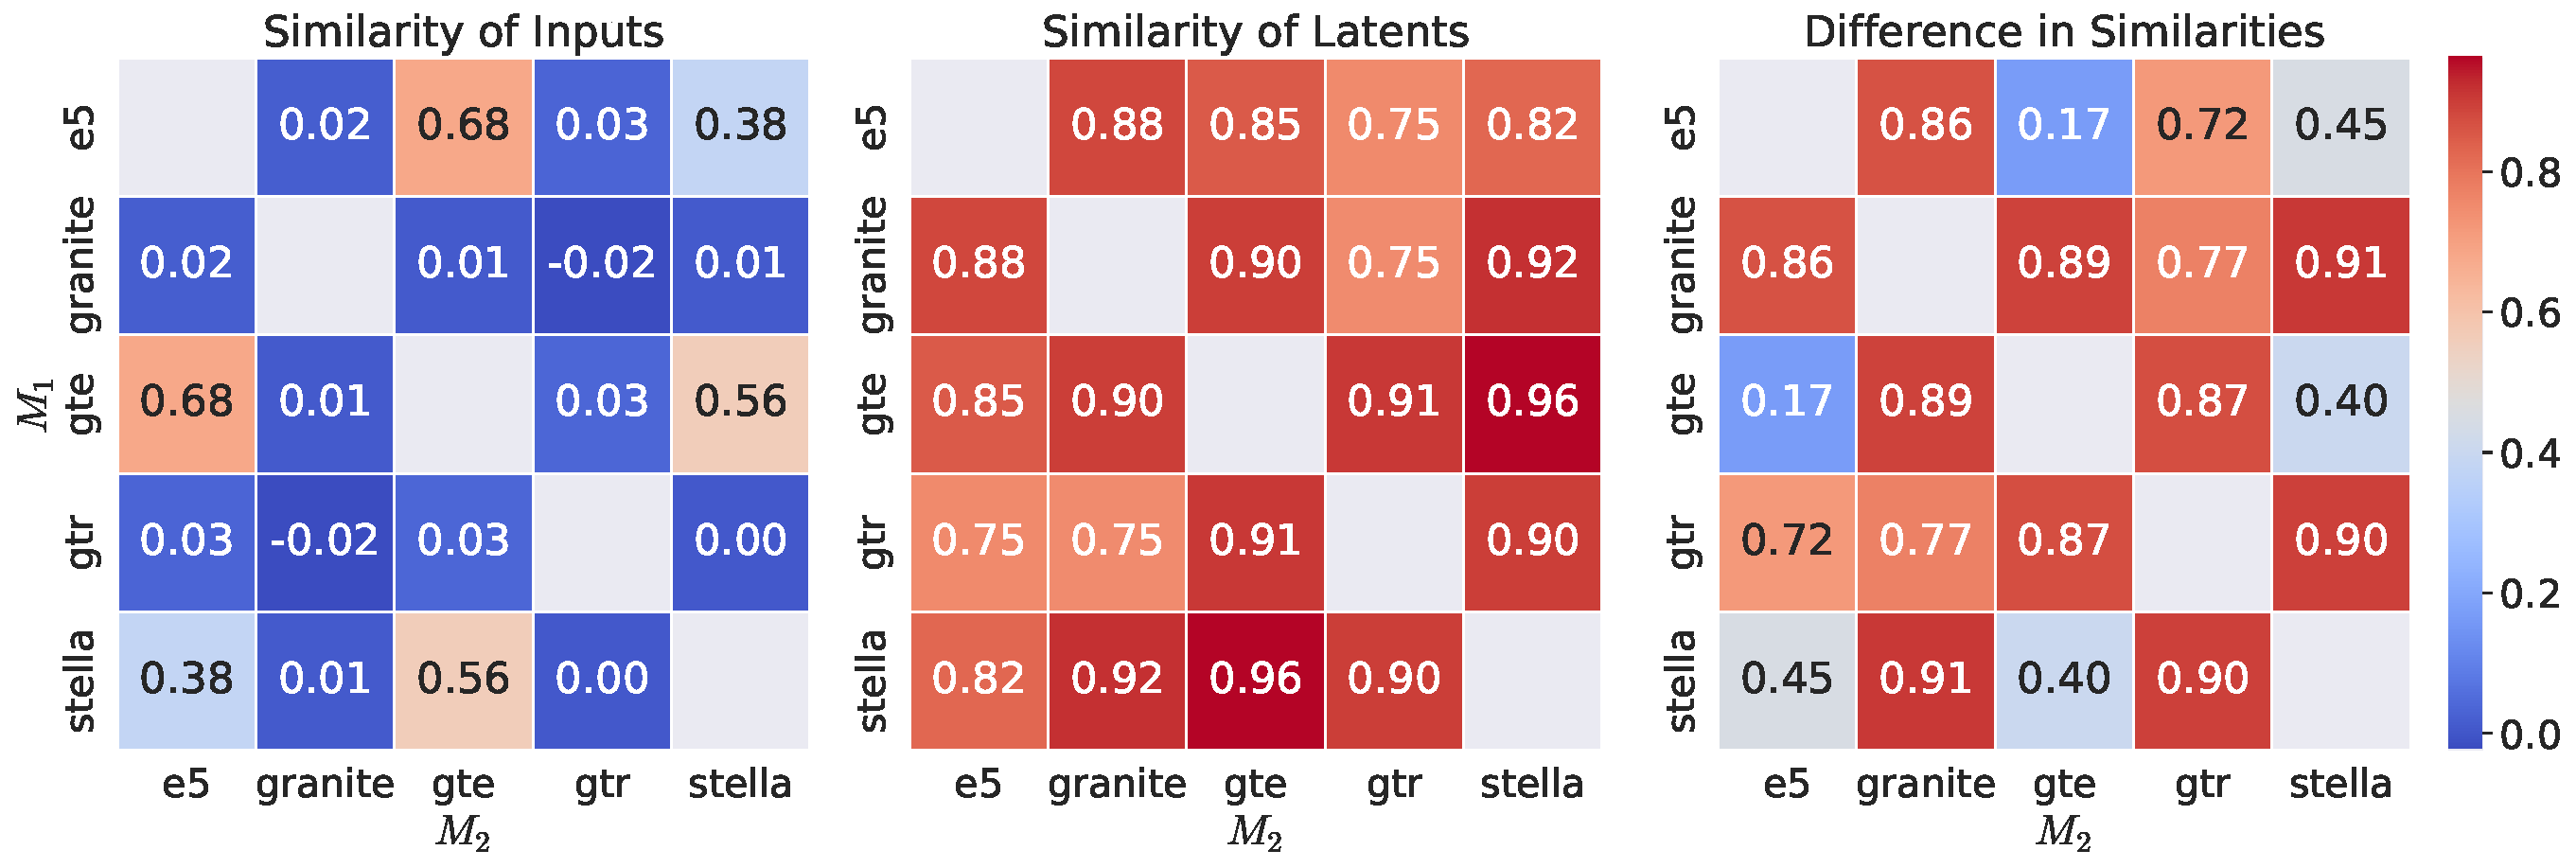
\includegraphics[width=\linewidth]{ims/cosine_heatmaps.pdf}
    \caption{Pairwise cosine similarities of input embeddings (left) and their \atk{} latents (middle) across different embedding pairs. The absolute difference between the heatmaps plots is on the right. All numbers are computed on the same batch of 1024 NQ texts.}
    \label{fig:cosine_heatmaps}
\end{figure}

\shortpara{\atk{} learns a universal latent space.}
\atk{} projects embeddings $M_{1,2,\ldots}$ into a shared latent space via compositions of input adapters ($A_{1,2,\ldots}$) and a shared translator $T$.  \Cref{fig:cosine_heatmaps} shows that even when the embeddings $u_i = M_1(d_i)$ and $v_i = M_2(d_i)$ are far apart (\textit{i.e.,} have low cosine similarity), their representations in \atk{}'s latent space are incredibly close: $T(A_1(u_i)) \approx T(A_2(v_i))$.  \Cref{fig:main} visualizes this (via two-dimensional projections) for \atk{} trained on gte and gtr embeddings: the embeddings are far apart, but their latents 
are \emph{nearly overlapping}.

% As we'll show in the rest of this paper, when passed through output adapters $B_1$ and $B_2$, these nearly-identical latents preserve \textit{geometry and semantics}. So, it follows that the shared latent space must entirely encode the geometric structure of the original embeddings, \textbf{thereby constructing a universal language of text encoders}.

% \vs{To convey the coolness, emphasize that it is not obvious that such a shared latent representation exists and even if it exists, it is not a priori obvious it is possible to discover.}

% \vs{You can also \textbf{start} with baselines, which helps emphasize that naive approaches fail.}


\begin{table}[!b]
    \scriptsize
    \centering
    \begin{tabular}{llrrrrrrrr}
    % \begin{tabular}{ll>{\columncolor{blue!10}}r>{\columncolor{blue!10}}r>{\columncolor{blue!10}}rrrrrrr}
        \toprule
        \multicolumn{2}{c}{} & \multicolumn{3}{c}{\atk{}} & \multicolumn{3}{c}{Naïve Baseline} & \multicolumn{2}{c}{OA Baseline}\\
        \cmidrule(lr){3-5} \cmidrule(lr){6-8}  \cmidrule(lr){9-10} 
        $M_1$ & $M_2$ & $\cos(\cdot)$ $\uparrow$ & Top-1 $\uparrow$ & Rank $\downarrow$ & $\cos(\cdot)$ $\uparrow$ & Top-1 $\uparrow$ & Rank $\downarrow$ & Top-1 $\uparrow$ & Rank $\downarrow$\\
        \midrule
        \multirow{4}{*}{gran.} & gtr & \textbf{0.80 {\tiny (0.0)}} & \textbf{0.99} & \textbf{1.19 {\tiny (0.1)}} & -0.03 {\tiny (0.0)} & 0.00 & 4168.73 {\tiny (9.2)} & 0.00 & 4096.75 {\tiny (9.2)} \\
         & gte & \textbf{0.87 {\tiny (0.0)}} & \textbf{0.95} & \textbf{1.18 {\tiny (0.0)}} & 0.01 {\tiny (0.0)} & 0.00 & 4088.58 {\tiny (9.2)} & 0.00 & 4069.91 {\tiny (9.2)} \\
         & stel. & \textbf{0.79 {\tiny (0.0)}} & \textbf{0.98} & \textbf{1.05 {\tiny (0.0)}} & 0.01 {\tiny (0.0)} & 0.00 & 4208.26 {\tiny (9.2)} & 0.00 & 4096.75 {\tiny (9.2)} \\
         & e5 & \textbf{0.85 {\tiny (0.0)}} & \textbf{0.98} & \textbf{1.11 {\tiny (0.0)}} & 0.02 {\tiny (0.0)} & 0.00 & 4111.60 {\tiny (9.2)} & 0.00 & 4096.75 {\tiny (9.2)} \\
        \midrule
        \multirow{4}{*}{gtr} & gran. & \textbf{0.81 {\tiny (0.0)}} & \textbf{0.99} & \textbf{1.02 {\tiny (0.0)}} & -0.03 {\tiny (0.0)} & 0.00 & 4169.76 {\tiny (9.2)} & 0.00 & 4096.66 {\tiny (9.2)} \\
         & gte & \textbf{0.87 {\tiny (0.0)}} & \textbf{0.93} & \textbf{2.31 {\tiny (0.1)}} & 0.04 {\tiny (0.0)} & 0.00 & 4080.92 {\tiny (9.2)} & 0.00 & 4079.92 {\tiny (9.2)} \\
         & stel. & \textbf{0.80 {\tiny (0.0)}} & \textbf{0.99} & \textbf{1.03 {\tiny (0.0)}} & 0.00 {\tiny (0.0)} & 0.00 & 4198.78 {\tiny (9.2)} & 0.00 & 4096.69 {\tiny (9.2)} \\
         & e5 & \textbf{0.83 {\tiny (0.0)}} & \textbf{0.84} & \textbf{2.88 {\tiny (0.2)}} & 0.03 {\tiny (0.0)} & 0.00 & 4082.84 {\tiny (9.2)} & 0.00 & 4066.42 {\tiny (9.2)} \\
        \midrule
        \multirow{4}{*}{gte} & gran. & \textbf{0.75 {\tiny (0.0)}} & \textbf{0.95} & \textbf{1.22 {\tiny (0.0)}} & 0.01 {\tiny (0.0)} & 0.00 & 4079.81 {\tiny (9.3)} & 0.00 & 4069.23 {\tiny (9.2)} \\
         & gtr & \textbf{0.75 {\tiny (0.0)}} & \textbf{0.91} & \textbf{2.64 {\tiny (0.1)}} & 0.04 {\tiny (0.0)} & 0.00 & 4084.15 {\tiny (9.2)} & 0.00 & 4078.45 {\tiny (9.2)} \\
         & stel. & \textbf{0.89 {\tiny (0.0)}} & \textbf{1.00} & \textbf{1.00 {\tiny (0.0)}} & 0.56 {\tiny (0.0)} & \textbf{1.00} &\textbf{ 1.00 {\tiny (0.0)}} & \textbf{1.00} & \textbf{1.00 {\tiny (0.0)}} \\
         & e5 & \textbf{0.87 {\tiny (0.0)}} & 0.99 & 5.19 {\tiny (0.5)} & 0.68 {\tiny (0.0)} & \textbf{1.00} &\textbf{ 1.00 {\tiny (0.0)}} & \textbf{1.00} & \textbf{1.00 {\tiny (0.0)}} \\
        \midrule
        \multirow{4}{*}{stel.} & gran. & \textbf{0.80 {\tiny (0.0)}} & \textbf{0.98} & \textbf{1.08 {\tiny (0.0)}} & 0.01 {\tiny (0.0)} & 0.00 & 4209.08 {\tiny (9.3)} & 0.00 & 4096.88 {\tiny (9.2)} \\
         & gtr & \textbf{0.82 {\tiny (0.0)}} & \textbf{1.00} & \textbf{1.10 {\tiny (0.0)}} & 0.00 {\tiny (0.0)} & 0.00 & 4192.31 {\tiny (9.2)} & 0.00 & 4096.63 {\tiny (9.2)} \\
         & gte & \textbf{0.92 {\tiny (0.0)}} & \textbf{1.00} & \textbf{1.00 {\tiny (0.0)}} & 0.56 {\tiny (0.0)} & \textbf{1.00} & \textbf{1.00 {\tiny (0.0)}} & \textbf{1.00} & \textbf{1.00 {\tiny (0.0)}} \\
         & e5 & \textbf{0.86 {\tiny (0.0)}} & \textbf{1.00} & \textbf{1.00 {\tiny (0.0)}} & 0.38 {\tiny (0.0)} & 0.99 & 1.03 {\tiny (0.0)} & \textbf{1.00} & \textbf{1.00 {\tiny (0.0)}} \\
        \midrule
        \multirow{4}{*}{e5} & gran. & \textbf{0.81 {\tiny (0.0)}} & \textbf{0.99} & \textbf{2.20 {\tiny (0.2)}} & 0.02 {\tiny (0.0)} & 0.00 & 4120.60 {\tiny (9.3)} & 0.00 & 4096.36 {\tiny (9.2)} \\
         & gtr & \textbf{0.74 {\tiny (0.0)}} & \textbf{0.82} & \textbf{2.56 {\tiny (0.0)}} & 0.03 {\tiny (0.0)} & 0.00 & 4080.76 {\tiny (9.3)} & 0.00 & 4065.74 {\tiny (9.2)} \\
         & gte & \textbf{0.90 {\tiny (0.0)}} & \textbf{1.00} & 1.01 {\tiny (0.0)} & 0.68 {\tiny (0.0)} & \textbf{1.00} & \textbf{1.00 {\tiny (0.0)}} & \textbf{1.00} & \textbf{1.00 {\tiny (0.0)}} \\
         & stel. & \textbf{0.78 {\tiny (0.0)}} & \textbf{1.00} & \textbf{1.00 {\tiny (0.0)}} & 0.38 {\tiny (0.0)} & \textbf{1.00} & \textbf{1.00 {\tiny (0.0)}} & \textbf{1.00} & \textbf{1.00 {\tiny (0.0)}} \\
        \bottomrule\\[-1.6ex]
    \end{tabular}
    \caption{In-distribution translations: \atk{}s trained on NQ and evaluated on a 65536 text subset of NQ (chunked in batches of size 8192). The rank metric varies from 1 to 8192, thus 4096 corresponds to a random ordering. Since Optimal Assignment is a matching method, cosine distances are not applicable.  Standard errors are shown in parentheses. Bold denotes best value.}
    \label{tab:embedding_comparison}
\end{table}

\shortpara{\atk{} translations mirror target geometry.}
\Cref{tab:embedding_comparison} shows that \atk{} generates embeddings with near-optimal assignment across model pairs, achieving cosine similarity scores up to 0.92, top-1 accuracies up to 100\%, and ranks as low as 1. In same-backbone pairings (e.g., (gte, e5)), \atk{}'s top-1 accuracy and rank are comparable to both the naïve baseline and (surprisingly) the oracle-aided optimal assignment. Although the embeddings generated by \atk{} are significantly closer to the ground truth than the naïve baseline, in same-backbone pairings the embeddings are close enough to be compatible.  In cross-backbone pairings, \atk{} is far superior on all metrics, while baseline methods perform similarly to random guessing.

% In particular, given that the evaluation set is chunked in batches of size $8192$ (for computational efficiency), the baseline methods' performance is no better than random in cross-backbone scenarios. This suggests that conventional matching approaches fail to capture structural relationships between embedding spaces unless initial cosine similarities are already sufficiently high.

% \vs{You train on a million embeddings but measure on 8000.  A few words would be helpful + mention that your test set is disjoint from training (is it?)}


\begin{table}[t]
    \scriptsize
    \centering
    \begin{tabular}{llrrr|rrr}
        \toprule
        \multicolumn{2}{c}{} & \multicolumn{3}{c}{TweetTopic} & \multicolumn{3}{c}{MIMIC}\\
        \cmidrule(lr){3-5} \cmidrule(lr){6-8}
        $M_1$ & $M_2$ & $\cos(\cdot)$ $\uparrow$& Top-1 $\uparrow$& Rank $\downarrow$& $\cos(\cdot)$ $\uparrow$& Top-1 $\uparrow$& Rank $\downarrow$\\
        \midrule
        \multirow{4}{*}{gran.} & gtr & 0.74 {\tiny (0.0)} & 0.99 & 1.09 {\tiny (0.1)} & 0.74 {\tiny (0.0)} & 0.60 & 23.38 {\tiny (1.6)} \\
        & gte & 0.85 {\tiny (0.0)} & 0.95 & 1.26 {\tiny (0.1)} & 0.85 {\tiny (0.0)} & 0.08 & 346.21 {\tiny (7.8)} \\
        & stel. & 0.77 {\tiny (0.0)} & 0.96 & 1.11 {\tiny (0.0)} & 0.72 {\tiny (0.0)} & 0.13 & 242.23 {\tiny (6.1)} \\
        & e5 & 0.83 {\tiny (0.0)} & 0.87 & 3.10 {\tiny (0.7)} & 0.84 {\tiny (0.0)} & 0.12 & 361.06 {\tiny (8.7)} \\
        \midrule
        \multirow{4}{*}{gtr} & gran. & 0.79 {\tiny (0.0)} & 0.98 & 2.41 {\tiny (0.6)} & 0.78 {\tiny (0.0)} & 0.51 & 35.27 {\tiny (1.9)} \\
        & gte & 0.85 {\tiny (0.0)} & 0.96 & 1.29 {\tiny (0.2)} & 0.84 {\tiny (0.0)} & 0.12 & 279.56 {\tiny (6.9)} \\
        & stel. & 0.77 {\tiny (0.0)} & 0.96 & 1.10 {\tiny (0.0)} & 0.72 {\tiny (0.0)} & 0.27 & 127.92 {\tiny (4.4)} \\
        & e5 & 0.80 {\tiny (0.0)} & 0.53 & 13.38 {\tiny (1.2)} & 0.82 {\tiny (0.0)} & 0.01 & 1413.80 {\tiny (18.3)} \\
        \midrule
        \multirow{4}{*}{gte} & gran. & 0.73 {\tiny (0.0)} & 0.94 & 1.33 {\tiny (0.1)} & 0.73 {\tiny (0.0)} & 0.09 & 342.15 {\tiny (7.8)} \\
        & gtr & 0.71 {\tiny (0.0)} & 0.95 & 1.29 {\tiny (0.1)} & 0.69 {\tiny (0.0)} & 0.12 & 256.63 {\tiny (6.4)} \\
        & stel. & 0.86 {\tiny (0.0)} & 1.00 & 1.00 {\tiny (0.0)} & 0.85 {\tiny (0.0)} & 1.00 & 1.00 {\tiny (0.0)} \\
        & e5 & 0.83 {\tiny (0.0)} & 0.91 & 1.57 {\tiny (0.2)} & 0.86 {\tiny (0.0)} & 0.54 & 17.71 {\tiny (0.9)} \\
        \midrule
        \multirow{4}{*}{stel.} & gran. & 0.79 {\tiny (0.0)} & 0.99 & 1.09 {\tiny (0.1)} & 0.77 {\tiny (0.0)} & 0.14 & 221.95 {\tiny (5.9)} \\
        & gtr & 0.77 {\tiny (0.0)} & 1.00 & 1.00 {\tiny (0.0)} & 0.75 {\tiny (0.0)} & 0.56 & 17.70 {\tiny (1.0)} \\
        & gte & 0.90 {\tiny (0.0)} & 1.00 & 1.00 {\tiny (0.0)} & 0.91 {\tiny (0.0)} & 1.00 & 1.00 {\tiny (0.0)} \\
        & e5 & 0.85 {\tiny (0.0)} & 0.98 & 1.05 {\tiny (0.0)} & 0.85 {\tiny (0.0)} & 0.51 & 26.33 {\tiny (1.2)} \\
        \midrule
        \multirow{4}{*}{e5} & gran. & 0.79 {\tiny (0.0)} & 0.98 & 1.08 {\tiny (0.0)} & 0.78 {\tiny (0.0)} & 0.21 & 151.09 {\tiny (4.6)} \\
        & gtr & 0.67 {\tiny (0.0)} & 0.80 & 3.10 {\tiny (0.6)} & 0.66 {\tiny (0.0)} & 0.01 & 1029.64 {\tiny (14.9)} \\
        & gte & 0.87 {\tiny (0.0)} & 0.99 & 1.02 {\tiny (0.0)} & 0.87 {\tiny (0.0)} & 0.60 & 32.59 {\tiny (2.6)} \\
        & stel. & 0.75 {\tiny (0.0)} & 0.98 & 1.06 {\tiny (0.0)} & 0.75 {\tiny (0.0)} & 0.46 & 32.12 {\tiny (1.4)} \\
        \bottomrule\\[-1.6ex]
    \end{tabular}
    \caption{Out-of-distribution translations: \atk{}s trained on NQ and evaluated on the entire TweetTopic test set (800 tweets) and an 8192-record subset of MIMIC. The rank metric varies from 1 to 800 (for TweetTopic) and 8192 (for MIMIC), thus 400 and, respectively, 4096 correspond to a random ordering. Standard errors are shown in parentheses.}
    \label{tab:embeddings_ood}
\end{table}

\Cref{tab:embeddings_ood} shows that this performance extends to out-of-distribution data.  Our \atk{} translators were trained on NQ (drawn from Wikipedia), yet exhibit high cosine similarity, high accuracy, and low rank when evaluated on tweets (which are far more colloquial and use emojis) and medical records (which contain domain-specific jargon unlikely to appear in NQ). In \Cref{sec:full_ood}, we show that baseline methods fail on cross-backbone embedding pairs.


\begin{table}[!b]
    \scriptsize
    \centering
    \begin{tabular}{llrrrrr}
        \toprule
        \multicolumn{2}{c}{} & \multicolumn{3}{c}{\atk{}} & \multicolumn{2}{c}{OA Baseline}\\
        \cmidrule(lr){3-5} \cmidrule(lr){6-7}
        $M_1$ & $M_2$ & $\cos(\cdot)$ $\uparrow$& Top-1 $\uparrow$& Rank $\downarrow$& Top-1 $\uparrow$& Rank $\downarrow$\\
        \midrule
        gran. & \multirow{5}{*}{clip} & \textbf{0.78 {\tiny (0.0)}} & \textbf{0.35} & \textbf{226.62} {\tiny (3.2)} & 0.00 & 4096.32 {\tiny (9.2)}\\
        gtr & & \textbf{0.73 {\tiny (0.0)}} & \textbf{0.13} & \textbf{711.23} {\tiny (5.9)} & 0.00 & 4096.71 {\tiny (9.2)} \\
        gte & & \textbf{0.62 {\tiny (0.0)}} & \textbf{0.00} & \textbf{3233.41} {\tiny (9.8)} & 0.00 & 4096.32 {\tiny (9.2)}\\
        stel. & & \textbf{0.77 {\tiny (0.0)}} & \textbf{0.31} & \textbf{286.69} {\tiny (3.6)} & 0.00 & 4096.60 {\tiny (9.2)} \\
        e5 & & \textbf{0.64 {\tiny (0.0)}} & \textbf{0.01} & \textbf{2568.21} {\tiny (9.4)} & 0.00 & 4096.78 {\tiny (9.2)}\\
        \midrule
        \multirow{5}{*}{clip} & gran. & \textbf{0.74 {\tiny (0.0)}} & \textbf{0.72} & \textbf{4.46} {\tiny (0.1)} & 0.00 & 4096.36 {\tiny (9.2)} \\
         & gtr & \textbf{0.67 {\tiny (0.0)}} & \textbf{0.27} & \textbf{155.11} {\tiny (2.1)} & 0.00 & 4096.80 {\tiny (9.2)} \\
         & gte & \textbf{0.75 {\tiny (0.0)}} & \textbf{0.00} & \textbf{2678.90} {\tiny (8.9)} & 0.00 & 4096.12 {\tiny (9.2)} \\
         & stel. & \textbf{0.72 {\tiny (0.0)}} & \textbf{0.61} & \textbf{22.50} {\tiny (0.5)} & 0.00 & 4096.47 {\tiny (9.2)} \\
         & e5 & \textbf{0.73 {\tiny (0.0)}} & \textbf{0.01} & \textbf{1692.28} {\tiny (8.2)} & 0.00 & 4096.44 {\tiny (9.2)} \\
        \bottomrule\\[-1.6ex]
    \end{tabular}
    \caption{Translations between unimodal and multimodal (CLIP) embeddings: \atk{}s trained on NQ and evaluated on a 65536 text subset of NQ (chunked in batches of size 8192). Rank varies from 1 to 8192, thus 4096 corresponds to a random ordering. Since the embedding dimensionalities are different, the naive baseline does not apply. Bold denotes best value.}
    \label{tab:CLIP_nq}
\end{table} 

Finally, \Cref{tab:CLIP_nq} shows that \atk{} can even translate to and from the space of CLIP, a multimodal embedding model which was trained in part on \emph{image} data.  While the translations are not as strong as in \Cref{tab:embedding_comparison}, \atk{} consistently outperforms the optimal assignment baseline. These results show that promise of our method at adapting to new modalities: in particular, the embedding space of CLIP has been successfully connected to other modalities such as heatmaps, audio, and depth charts \citep{girdhar2023imagebind}.

% Stronger methods and/or better hyperparameters may yield even better translations.  Alternatively, it may be possible to translate to and from CLIP using granite or stella as intermediate representations. We leave this to future work.



% \begin{figure}[h]
%     \centering
%     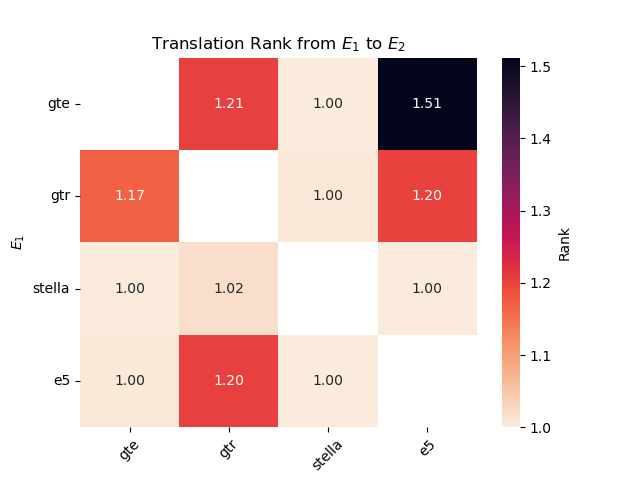
\includegraphics[width=0.6\linewidth]{ims/heatmap_nq.png}
%     \caption{NQ Rank}
%     \label{fig:nq}
% \end{figure}


%%%%%%%%%%%%%%%%%%%% SECTION BREAK %%%%%%%%%%%%%%%%%%%%

\section{Using \atk{} translations to extract information}
\label{sec:eval_semantics}

In this section, we show that \atk{} translations not only preserve the geometric structure of embeddings but also retain sufficient semantics to enable attribute inference.

% In \Cref{sec:eval_geometry} we demonstrated that \atk{} translations faithfully preserve geometric structure. In this section, we extend that result to show that they additionally retain the semantics of the original source embeddings: a capability that has important security implications. 

%Vector databases underpin modern search by indexing data as embeddings. In a breach of such a system where the encoder and any input–embedding pairs are unknown, we show that attackers can \textit{still} extract sensitive information from raw vectors \textit{with no other knowledge}.


\begin{table}[!t]
    \scriptsize
    \centering
    \begin{tabular}{llcccc|cccc}
        \toprule
        \multicolumn{2}{c}{} & \multicolumn{4}{c}{TweetTopic ($k=1$)} & \multicolumn{4}{c}{MIMIC ($k=10$)}\\
        \cmidrule(lr){3-6} \cmidrule(lr){7-10}
        $M_1$ & $M_2$ & \atk{} & Naïve & $M_1$ & $M_2$ & \atk{} & Naïve & $M_1$ & $M_2$ \\
        \midrule
        \multirow{4}{*}{gran.} & gtr & 0.25 & 0.10 & 0.30 & 0.24 & 0.19 & 0.11 & 0.76 & 0.88 \\
        & gte & 0.32 & 0.09 & 0.30 & 0.34 & 0.36 & 0.13 & 0.76 & 1.00 \\
        & stel. & 0.24 & 0.10 & 0.30 & 0.28 & 0.27 & 0.04 & 0.76 & 0.96 \\
        & e5 & 0.31 & 0.18 & 0.30 & 0.31 & 0.19 & 0.20 & 0.76 & 0.97 \\
        \midrule
        \multirow{4}{*}{gtr} & gran. & 0.34 & 0.08 & 0.24 & 0.30 & 0.16 & 0.12 & 0.88 & 0.76 \\
        & gte & 0.33 & 0.13 & 0.24 & 0.34 & 0.28 & 0.05 & 0.88 & 1.00 \\
        & stel. & 0.30 & 0.10 & 0.24 & 0.28 & 0.25 & 0.07 & 0.88 & 0.96 \\
        & e5 & 0.30 & 0.04 & 0.24 & 0.31 & 0.09 & 0.09 & 0.88 & 0.97 \\
        \midrule
        \multirow{4}{*}{gte} & gran. & 0.37 & 0.04 & 0.34 & 0.30 & 0.18 & 0.11 & 1.00 & 0.76 \\
        & gtr & 0.24 & 0.13 & 0.34 & 0.24 & 0.10 & 0.03 & 1.00 & 0.88 \\
        & stel. & 0.31 & 0.20 & 0.34 & 0.28 & 0.68 & 0.83 & 1.00 & 0.96 \\
        & e5 & 0.37 & 0.30 & 0.34 & 0.31 & 0.37 & 0.63 & 1.00 & 0.97 \\
        \midrule
        \multirow{4}{*}{stel.} & gran. & 0.35 & 0.07 & 0.28 & 0.30 & 0.23 & 0.09 & 0.96 & 0.76 \\
        & gtr & 0.26 & 0.13 & 0.28 & 0.24 & 0.22 & 0.09 & 0.96 & 0.88 \\
        & gte & 0.38 & 0.36 & 0.28 & 0.34 & 0.90 & 0.98 & 0.96 & 1.00 \\
        & e5 & 0.35 & 0.34 & 0.28 & 0.31 & 0.38 & 0.46 & 0.96 & 0.97 \\
        \midrule
        \multirow{4}{*}{e5} & gran. & 0.33 & 0.15 & 0.31 & 0.30 & 0.14 & 0.07 & 0.97 & 0.76 \\
        & gtr & 0.26 & 0.22 & 0.31 & 0.24 & 0.11 & 0.04 & 0.97 & 0.88 \\
        & gte & 0.34 & 0.28 & 0.31 & 0.34 & 0.47 & 0.66 & 0.97 & 1.00 \\
        & stel. & 0.26 & 0.16 & 0.31 & 0.28 & 0.36 & 0.40 & 0.97 & 0.96 \\
        \bottomrule\\[-1.6ex]
    \end{tabular}
    \caption{Information leakage via top-$k$ zero-shot attribute inference: \atk{}s trained on NQ and evaluated on the TweetTopic test set (800 tweets) and an 8192-record subset of MIMIC. $M_1$ and $M_2$ represent \textit{ideal} zero-shot inference: attributes and embeddings are encoded using the same model.}
    \label{tab:tweet_topic_mimic_class}
\end{table}


\begin{wrapfigure}{r}{0.42\textwidth}
    \centering
    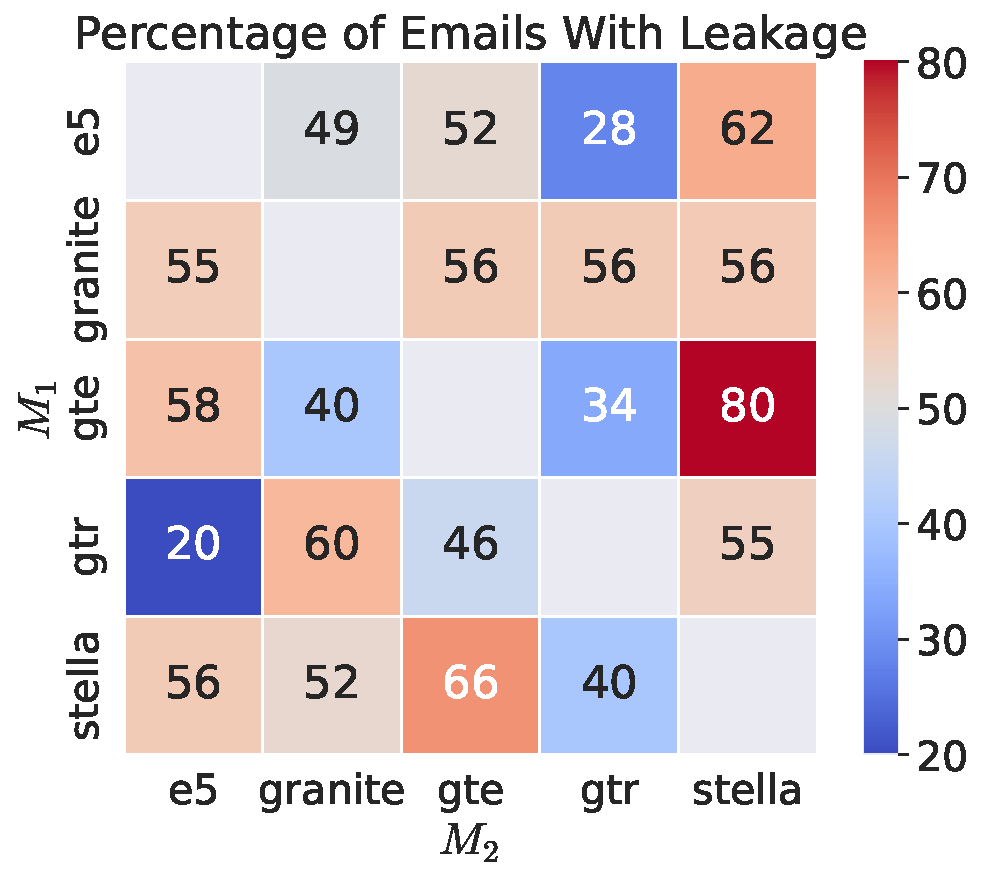
\includegraphics[width=0.37\textwidth]{ims/enron_heatmap.pdf}
      \caption{Leakage of information via inversion. Trained on NQ and evaluated on a 50-email subset of the Enron Email Corpus. Cells denote judge accuracy.}
    \label{fig:enron_heatmap}
\end{wrapfigure}

\shortpara{Zero-shot attribute inference.}
\label{sec:tweet_classification}
\Cref{tab:tweet_topic_mimic_class} shows that attribute inference on \atk{} translations consistently outperforms the naïve baseline and often does better than the ideal zero-shot baseline which performs inference on ground-truth document and attribute embeddings in the same space (this baseline is imaginary since these embeddings are not available in our setting).


% despite translating out-of-distribution tweets, \atk{} preserves sufficient semantic information from the original embedding space to enable effective zero-shot attribute extraction. In fact, attribute extraction from our translated embeddings consistently outperforms the  and frequently surpasses even hypothetical zero-shot extractions performed directly on the untranslated source or target embeddings. We hypothesize that this improved performance arises because the universal latent space captures and integrates shared knowledge from both embedding spaces.


% \paragraph{Case study: extracting disease information from medical records}
\label{sec:mimic_classification}
\atk{} translations even work for embeddings of medical records, which are much further from the training distribution than tweets.  The attributes in this case are MedCAT disease descriptions, very few of which occur in the training data.  Attribute inference on translated embeddings is comparable to the naïve baseline in same-backbone pairings and outperforms it (often greatly) in cross-backbone pairings.  The fact that \atk{} preserves the semantics of concepts like "alveolar periostitis" (which never appears in its training data) is evidence that its latent space is indeed a universal representation.



% \begin{figure}[t]
%     \centering
%     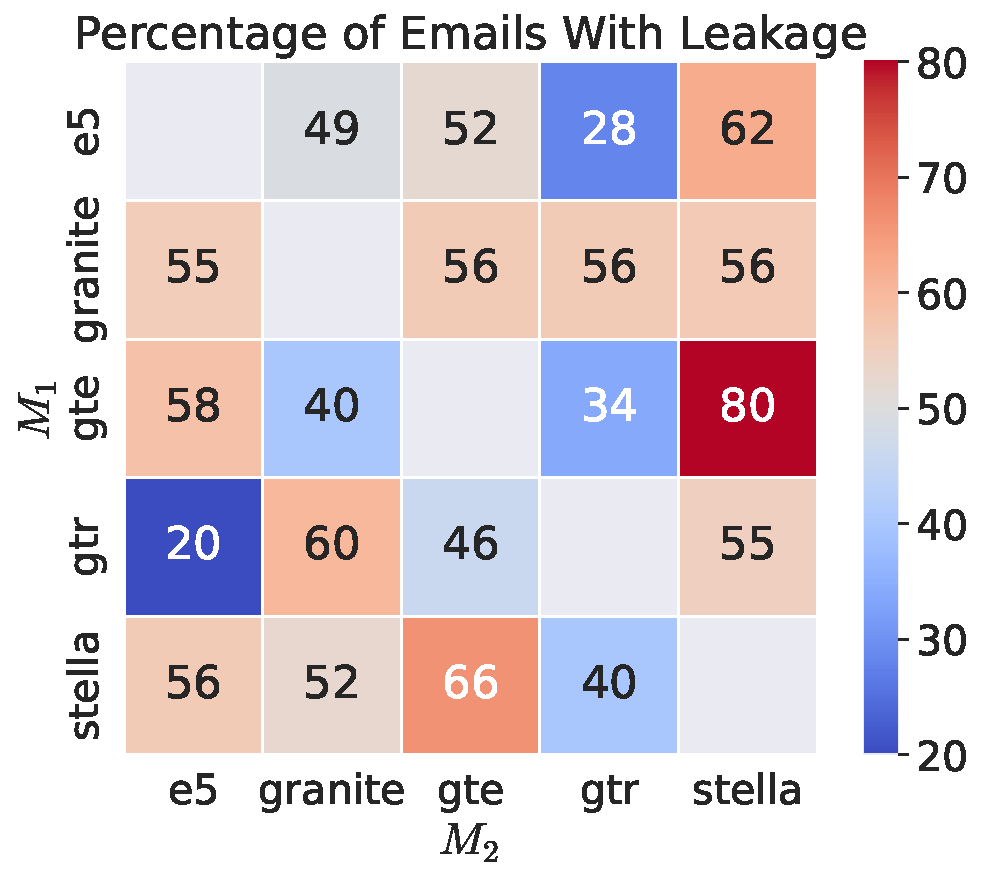
\includegraphics[width=0.5\linewidth]{ims/enron_heatmap.pdf}
%     \caption{Measuring the leakage of information via embedding inversion. \atk{}s trained on NQ and evaluated on a 50-email subset of the Enron Email Corpus. Each cell represents the percentage of reconstructed emails that an LLM judge decided leaked information.}
%     \label{fig:enron_heatmap}
% \end{figure}

\shortpara{Zero-shot inversion.}
Inversion, i.e., reconstruction of text inputs, is more ambitious than attribute inference.  \atk{} translations retain enough semantic information that off-the-shelf, zero-shot inversion methods like~\cite{zhang2025universalzeroshotembeddinginversion}, developed for embeddings computed by standard encoders, extract information for as many as 80\% of documents given \emph{only} their translated embeddings, for some model pairs (\Cref{fig:enron_heatmap}).  These inversions are imperfect and we leave development of specialized inverters for translated embeddings to future work.  Nevertheless, as exemplified in \Cref{fig:inversion_example}, they still extract information such as individual and company names, dates, promotions, financial information, outages, and even lunch orders. In \Cref{sec:prompt}, we show the prompt we use to measure extraction.

\begin{figure}[ht]
  \centering
    \begin{callout}
    \textbf{Ground Truth:} ``Subject: \colorbox{green}{Enron} \colorbox{yellow}{Bashing} on Frontline \verb|\n| Body:..."\\
    \textbf{Generation:} ``Some emails discussing \colorbox{green}{NROn} Employee/s \colorbox{yellow}{Complaint To thePublic}..."\\
    
    \textbf{Ground Truth:} ``Subject: \colorbox{yellow}{Trades for 3/1/02} \verb|\n| Body: \verb|\n| \colorbox{green}{John}, \verb|\n| The following trades..."\\
    \textbf{Generation:} ``... \colorbox{yellow}{future transactions} may await \colorbox{green}{John} G..."\\

    \textbf{Ground Truth:} ``\colorbox{yellow}{The following expense report} is ready for approval..."\\
    \textbf{Generation:} ``\colorbox{yellow}{The upcoming expense statement} from YYYY MM Dec..."    
    \end{callout}
  \caption{Examples of inversions that infer \colorbox{green}{entities} and \colorbox{yellow}{content}.}
  \label{fig:inversion_example}
\end{figure}







% e5 -> gte: 52\%
% \begin{verbatim}
% {
%     "ground_truth": "Subject: \n Body: \n IMPORTANT MESSAGE! PLEASE READ! \n FILENET SYSTEM OUTAGE \n NOVEMBER 30, 2001 \n The FileNET System will be down for offline backups beginning today, November 30th at 5:00pm",
%     "generation": "Today's computers encountered an abrupt stop during communications and affected customer synchronization dates as scheduled backups of critical business information had their timestamp outlastd until after service reactivation",
% },
% \end{verbatim}

% gte -> gtr: 34\%



% Old data:
% \begin{table}[h]
%     \centering
%     \begin{tabular}{llccc|cc|ccc}
%         \toprule
%         \multicolumn{2}{c}{} & \multicolumn{3}{c}{Embedding} & \multicolumn{2}{c}{Text Inversion} & \multicolumn{3}{c}{Extraction (Top-3)} \\
%         \cmidrule(lr){3-5} \cmidrule(lr){6-7} \cmidrule(lr){8-10}
%         $E_1$ & $E_2$ & $\cos(\cdot)$ & Top-1 & Rank & $\cos(\cdot)$ & Token-F1 & $E_1 \to E_2$ & $E_1$ & $E_2$ \\
%         \midrule
%         gte & gtr & 0.70 & 0.80 & 1.78 & 0.58 & 0.10 & 0.01 & 0.99 & 0.97 \\
%         gtr & gte & 0.83 & 0.76 & 2.33 & - & - & 0.01 & 0.97 & 0.99 \\
%         stella & gte & 0.90 & 1.00 & 1.00 & - & - & 0.43 & 0.89 & 0.99 \\
%         gte & stella & 0.86 & 1.00 & 1.00 & - & - & 0.27 & 0.99 & 0.89 \\
%         s-t5 & gtr & 0.85 & 1.00 & 1.00 & 0.67 & 0.14 & 0.83 & 0.92 & 0.97 \\
%         gtr & s-t5 & 0.93 & 1.00 & 1.00 & - & - & 0.67 & 0.97 & 0.92 \\
%         \bottomrule
%     \end{tabular}
%     \caption{Full name extraction! GANs trained on NQ and evaluated on Enron (out-of-distribution)}
%     \label{tab:embedding_comparison}
% \end{table}

\section{Related work}

% Slack message abouut RW: https://cornell-security.slack.com/archives/C05QFLQ25UZ/p1709748413419549

% We need to concisely explain what uses pairs, what uses words/images. Why no one 



\shortpara{Representation alignment.}
Similarities between representations of
different neural networks are investigated in \citep{laakso2000content, li2016convergentlearningdifferentneural, wang2018understandinglearningrepresentationsextent, bansal2021revisitingmodelstitchingcompare, huh2024platonicrepresentationhypothesis}. CCA \citep{morcos2018insightsrepresentationalsimilarityneural}, SVCCA, \citep{raghu2017svccasingularvectorcanonical}, CKA \citep{kornblith2019similarity}, ICA \citep{yamagiwa2023discoveringuniversalgeometryembeddings}, and GUI-based systems such as embComp \citep{heimerl2019embComp} compare embeddings from different subspaces.  
Methods like \citep{maiorca2024latentspacetranslationsemantic, moschella2023relativerepresentationsenablezeroshot, moayeri2023texttoconceptandbackcrossmodel, norelli2023asifcoupleddataturns} harness representation similarity for zero-shot stitching, substitution, and multi-modal adaptation.  All rely on some amount of paired data, which is difficult  
to reduce \citep{cannistraci2023bootstrappingparallelanchorsrelative}.  Our method does not just measure similarity, we learn how to \emph{translate} representations across spaces without any paired data.

% between the two modalities of interest


\shortpara{Unsupervised transport.}  The problem of unsupervised transport has been studied for images \citep{huang2018multimodalunsupervisedimagetoimagetranslation, liu2018unsupervisedimagetoimagetranslationnetworks,zhu2020unpairedimagetoimagetranslationusing}, words \citep{xing2015normalized, conneau2018wordtranslationparalleldata, grave2018unsupervisedalignmentembeddingswasserstein, chen2018unsupervisedmultilingualwordembeddings}, and natural language sequences \citep{raviknight2011deciphering, lample2018unsupervisedmachinetranslationusing, alvarezmelis2018gromovwassersteinalignmentwordembedding, artetxe2018unsupervisedneuralmachinetranslation, yang2018unsupervisedneuralmachinetranslation}. Our method builds on these works, which often employ a combination of cycle-consistency and adversarial loss. \citep{schnaus2025itsblindmatchvisionlanguage} proposes a solver for matching small sets of embeddings between different vision-language models.  Our method goes well beyond matching by taking unknown embeddings and \emph{generating} matching embeddings in the space of another model.

% we directly translate embeddings from the space of one model to another in a way that generalizes to unseen embeddings.


% We note that this unsupervised mapping problem has a long history in machine learning, and research has successfully learned similar mapping functions between images, \citep{huang2018multimodalunsupervisedimagetoimagetranslation, liu2018unsupervisedimagetoimagetranslationnetworks,zhu2020unpairedimagetoimagetranslationusing}, words from different languages \citep{xing2015normalized, conneau2018wordtranslationparalleldata, grave2018unsupervisedalignmentembeddingswasserstein, chen2018unsupervisedmultilingualwordembeddings}, and even language sequences \citep{raviknight2011deciphering, lample2018unsupervisedmachinetranslationusing, artetxe2018unsupervisedneuralmachinetranslation}. Inspired by the success of adversarial methods in these problem settings, and the fact that embeddings from different models share latent structure \citep{huh2024platonicrepresentationhypothesis},


\shortpara{Embedding inversion.} An emerging line of research investigates decoding text from language model embeddings \citep{song2020informationleakageembeddingmodels, li2023sentenceembeddingleaksinformation, morris2023textembeddingsrevealalmost} and outputs \citep{morris2023languagemodelinversion, carlini2024stealingproductionlanguagemodel, zhang2024extractingpromptsinvertingllm}.  
\atk{} helps apply these to unknown embeddings, without an encoder or paired data, by translating them to the space of a known model. 

% (In one experiment, we evaluate the same inversion models from \citep{morris2023textembeddingsrevealalmost} on our translated pairs.)

% \paragraph{Upgrading embeddings.} A line of work in information retrieval builds embeddings that are \textit{backwards-compatible} with existing models \citep{shen2021backwardcompatiblerepresentationlearning, hu2022backwardcompatibleembeddings, ramanujan2022forwardcompatibletraininglargescale, jaeckle2023fastfillefficientcompatiblemodel, park2019relationalknowledgedistillation, wang2020unifiedrepresentationlearningcross}. We, instead, train an existing model for converting between a diverse set of embedding spaces. Other recent studies \citep{yoon2024matryoshkaadaptorunsupervisedsupervisedtuning, anonymous2024embeddingconverter} propose ways to improve or convert existing models; unlike these studies, we pretrain a large model for many-to-many conversion.

\shortpara{Bridging modality gaps.} Previous work has noted an inherent ``gap” between image- and text-based models \citep{liang2022mindgapunderstandingmodality} and proposed various ways to unify the modalities \citep{song2023bridgegapmodalitiescomprehensive}. Some approaches feed image embeddings directly into language models \citep{koh2023fromage, wang2023visionllm, dong2024dreamllmsynergisticmultimodalcomprehension, liu2023visualinstructiontuning}, while others generate captions from image embeddings \citep{mokady2021clipcap} or even from text embeddings themselves \citep{morris2023textembeddingsrevealalmost}. \citep{girdhar2023imagebind} introduces a shared embedding space that integrates inputs from multiple modalities, including text, audio, and vision. In contrast, our post-hoc approach directly translates between representations and complements these systems by enabling inputs from a wide variety of embedding models.
\section{Discussion and Future Work}

% The original Platonic Representation Hypothesis conjectures that the representation spaces of modern neural networks are converging. While the hypothesis itself is up for debate, it is even less obvious that there exists a method to explicitly discover such a universal representation. Remarkably, we demonstrate not only that this universal representation exists (across the encoders we study), but that it can be systematically constructed using our method.


% This robust in-distribution and out-of-distribution performance indicates that \atk{} does not just learn to translate its training embeddings but rather learns a domain‑agnostic mapping. By encoding the underlying semantics of models $M_1$ and $M_2$ into its shared latent space, our method learns a mathematical relationship between embedding spaces that transfers across diverse data distributions. This allows \atk{} to generate the correct embedding for input text it has never seen on an encoder it does not have access to, just by harnessing the universal geometry of embeddings.

% \atk{}’s strong performance on both in- and out-of-distribution data suggests it does more than memorize training translations---it learns the mathematical relationship between embedding spaces. By capturing the shared semantics of models $M_1$ and $M_2$ in a universal latent space, \atk{} can generate accurate target embeddings for unseen text from an encoder it has never encountered, purely by leveraging the universal geometry of embeddings.

% Importantly, we were able to extract sensitive attributes (disease information) from patient records \textit{with access to only their raw embeddings}, implying that a leak of hospital embeddings is equivalent to leakage of patient data. As translation methods like \atk{} improve, higher-fidelity extractions (perhaps of names, addresses, and other personal data) will become easier and more harmful. This trend necessitates that practitioners start to handle embeddings like they would handle their underlying text.

% The quality of inversions will improve dramatically with improvements in both translation and inversion. As such, we again emphasize the importance of treating embeddings safely---less like the raw numbers they appear as and more like the underlying texts they are functionally equivalent to.

% We emphasize that our method measures a \textit{lower bound} on the potential of inter-embedding translation, and any methodological improvements (including both better learning algorithms and better architectures) will improve our ability to translate between modalities. In particular, a class of more stable models would enable us to scale our system to more parameters and more data, likely improving our ability to translate in most settings.

% Our experiments relate to text-only embeddings as well as multimodal models like CLIP that include text as a modality. We see our results as empirical validation of the Platonic Representation Hypothesis \citep{huh2024platonicrepresentationhypothesis}, and look forward to other future work that extends our framework to new modalities and model families.

The Platonic Representation Hypothesis conjectures that the representation spaces of modern neural networks are converging.   We assert the Strong Platonic Representation Hypothesis: the latent universal representation can be learned and harnessed to translate between representation spaces without any encoders or paired data.

In \Cref{sec:eval_geometry}, we demonstrated 
that our \atk{} method successfully translates embeddings generated from unseen documents by unseen encoders, and the translator is robust to (sometimes very) out-of-distribution inputs.  This suggests that \atk{} learns domain-agnostic translations based on the universal geometric relationships which encode the same semantics in multiple embedding spaces.

% This suggests our method doesn't just memorize training examples but learns a domain-agnostic mapping that captures the underlying mathematical relationship between embedding spaces. By encoding the shared semantics of models $M_1$ and $M_2$ into a universal latent space, \atk{} can generate accurate target embeddings for unseen text from unfamiliar encoders by harnessing the universal geometry of embeddings.

In \Cref{sec:eval_semantics}, we showed that \atk{} translations preserve sufficient input semantics to enable attribute inference. 
We extracted sensitive disease information from patient records and partial content from corporate emails, with access only to document embeddings and no access to the encoder that produced them.  Better translation methods will enable higher-fidelity extraction, confirming once again that embeddings reveal (almost) as much as their inputs.

% We successfully extracted sensitive disease information from patient records and confidential information from business records with access only to their raw embeddings. This demonstrates that embedding leakage is functionally equivalent to leaking the underlying text itself. As translation methods like \atk{} improve, higher-fidelity extractions of personal data will become increasingly feasible, underscoring the importance of treating embeddings as sensitive as the texts they represent.

Our findings provide compelling evidence for the Strong Platonic Representation Hypothesis for text-based models.  Our preliminary results on CLIP suggest that the universal geometry can be harnessed in other modalities, too.  The results in this paper are but a \emph{lower bound} on inter-representation translation.  Better and more stable learning algorithms, architectures, and other methodological improvements will support scaling to more data, more model families, and more modalities.

% Based on our findings, we see our results as compelling evidence for both the original and Strong Platonic Representation Hypotheses for text-based models. Our preliminary results on CLIP further extend this perspective, leading us to conjecture that the full Strong Platonic Representation Hypothesis holds true. Importantly, our method demonstrates a \textit{lower bound} on the potential of inter-embedding translation, and any methodological improvements (including both better learning algorithms and architectures) will improve our ability to translate between modalities. In particular, a class of more stable models would enable us to scale our system to more parameters and more data, likely improving our ability to translate in most settings. We look forward to future work that extends our framework to new modalities and model families.
\input{sections/06_ablations}
% \input{sections/07_conclusion}

\begin{ack}

This research is supported in part by the Google Cyber NYC Institutional Research Program.
JM is supported by the National Science Foundation.

% Use unnumbered first level headings for the acknowledgments. All acknowledgments go at the end of the paper before the list of references. Moreover, you are required to declare funding (financial activities supporting the submitted work) and competing interests (related financial activities outside the submitted work). More information about this disclosure can be found at: \url{https://neurips.cc/Conferences/2025/PaperInformation/FundingDisclosure}.

% Do {\bf not} include this section in the anonymized submission, only in the final paper. You can use the \texttt{ack} environment provided in the style file to automatically hide this section in the anonymized submission.
\end{ack}

% \FloatBarrier
% {
%     \footnotesize
%     \setlength{\bibsep}{0pt plus 0.1ex} 
%     % \input{main.bbl}
%     \bibliography{main.bib}
%     \bibliographystyle{plainurl}
% }
\printbibliography

%%%%%%%%%%%%%%%%%%%%%%%%%%%%%%%%%%%%%%%%%%%%%%%%%%%%%%%%%%%%

\newpage
\appendix
\section{Compute}
Our training and evaluation were conducted using diverse compute environments, including both local and cloud GPU clusters. Experiments were done on NVIDIA 2080Ti, L4, A40, and A100 GPUs, listed in order of increasing computational capacity.

For our main experiments, we trained 36 distinct \atk{} models, with training durations ranging from 1 to 7 days per model, depending on the specific GPU and model pair (which affected convergence rates).  Additional 9 \atk{} models were trained for our ablations, bringing the total to 45 \atk{} models. Taking a conservative estimate of the average training time, this amounted to approximately 180 GPU days (45 models $\times$ 4 days / model).

Evaluation procedures varied by model type:
\begin{itemize}
    \item For each of our 45 \atk{} models, our full evaluation on NQ, TweetTopic, and MIMIC datasets required approximately 1 hour per model across all GPU types.
    \item The 36 non-ablation GANs underwent additional analysis on the Enron email corpus, requiring about 1.5 hours for inversion and downstream LLM evaluation.
    \item Naive baselines (30 models without CLIP) required approximately 30 minutes each for evaluation, roughly half the time needed for our full models.
    \item Optimal assignment baselines (36 models) were run exclusively on CPU. We implemented 4 different assignment algorithms, each requiring approximately 4 hours of computation time. The Gromov-Wasserstein algorithm was particularly computationally intensive and was included for CLIP due to dimensional differences.
\end{itemize}

In total, our experiments consumed approximately 180 GPU days for training and an additional 78 GPU hours for evaluation and analysis. There were approximately 144 CPU hours required for optimal assignment.



\section{Full out-of-distribution translation results}
\label{sec:full_ood}
We provide baseline numbers for the experiments shown in \Cref{tab:embeddings_ood}, by dataset.
\begin{table}[!ht]
    \scriptsize
    \centering
    \begin{tabular}{llrrrrrrrr}
        \toprule
        \multicolumn{2}{c}{} & \multicolumn{3}{c}{\atk{}} & \multicolumn{3}{c}{Naïve} & \multicolumn{2}{c}{Optimal Transport}\\
        \cmidrule(lr){3-5} \cmidrule(lr){6-8}  \cmidrule(lr){9-10} 
        $E_1$ & $E_2$ & $\cos(\cdot)$ & Top-1 & Rank & $\cos(\cdot)$ & Top-1 & Rank & Top-1 & Rank\\
        \midrule
        \multirow{4}{*}{gte} & gtr & 0.71 {\tiny (0.0)} & 0.95 & 1.29 {\tiny (0.1)} & 0.04 {\tiny (0.0)} & 0.00 & 386.58 {\tiny (8.3)} & 0.00 & 383.41 {\tiny (8.1)} \\
        & stel. & 0.86 {\tiny (0.0)} & 1.00 & 1.00 {\tiny (0.0)} & 0.58 {\tiny (0.0)} & 1.00 & 1.00 {\tiny (0.0)} & 1.00 & 1.00 {\tiny (0.0)} \\
        & e5 & 0.83 {\tiny (0.0)} & 0.91 & 1.57 {\tiny (0.2)} & 0.68 {\tiny (0.0)} & 1.00 & 1.00 {\tiny (0.0)} & 1.00 & 1.00 {\tiny (0.0)} \\
        & gran. & 0.73 {\tiny (0.0)} & 0.94 & 1.33 {\tiny (0.1)} & 0.00 {\tiny (0.0)} & 0.00 & 408.81 {\tiny (8.3)} & 0.01 & 398.16 {\tiny (8.2)} \\
        \midrule
        \multirow{4}{*}{gtr} & gte & 0.85 {\tiny (0.0)} & 0.96 & 1.29 {\tiny (0.2)} & 0.04 {\tiny (0.0)} & 0.00 & 392.01 {\tiny (8.2)} & 0.00 & 384.00 {\tiny (8.1)} \\
        & stel. & 0.77 {\tiny (0.0)} & 0.96 & 1.10 {\tiny (0.0)} & 0.00 {\tiny (0.0)} & 0.00 & 394.69 {\tiny (8.3)} & 0.00 & 390.67 {\tiny (8.2)} \\
        & e5 & 0.80 {\tiny (0.0)} & 0.53 & 13.38 {\tiny (1.2)} & 0.03 {\tiny (0.0)} & 0.00 & 400.85 {\tiny (8.2)} & 0.00 & 400.48 {\tiny (8.2)} \\
        & gran. & 0.79 {\tiny (0.0)} & 0.98 & 2.41 {\tiny (0.6)} & -0.04 {\tiny (0.0)} & 0.00 & 411.53 {\tiny (8.3)} & 0.00 & 401.01 {\tiny (8.2)} \\
        \midrule
        \multirow{4}{*}{stel.} & gte & 0.90 {\tiny (0.0)} & 1.00 & 1.00 {\tiny (0.0)} & 0.58 {\tiny (0.0)} & 1.00 & 1.00 {\tiny (0.0)} & 1.00 & 1.00 {\tiny (0.0)} \\
        & gtr & 0.77 {\tiny (0.0)} & 1.00 & 1.00 {\tiny (0.0)} & 0.00 {\tiny (0.0)} & 0.00 & 393.07 {\tiny (8.1)} & 0.00 & 390.26 {\tiny (8.2)} \\
        & e5 & 0.85 {\tiny (0.0)} & 0.98 & 1.05 {\tiny (0.0)} & 0.37 {\tiny (0.0)} & 0.89 & 1.55 {\tiny (0.1)} & 1.00 & 1.00 {\tiny (0.0)} \\
        & gran. & 0.79 {\tiny (0.0)} & 0.99 & 1.09 {\tiny (0.1)} & 0.00 {\tiny (0.0)} & 0.00 & 418.16 {\tiny (8.4)} & 0.00 & 400.95 {\tiny (8.2)} \\
        \midrule
        \multirow{4}{*}{e5} & gte & 0.87 {\tiny (0.0)} & 0.99 & 1.02 {\tiny (0.0)} & 0.68 {\tiny (0.0)} & 1.00 & 1.00 {\tiny (0.0)} & 1.00 & 1.00 {\tiny (0.0)} \\
        & gtr & 0.67 {\tiny (0.0)} & 0.80 & 3.10 {\tiny (0.6)} & 0.03 {\tiny (0.0)} & 0.00 & 401.16 {\tiny (8.4)} & 0.00 & 400.49 {\tiny (8.2)} \\
        & stel. & 0.75 {\tiny (0.0)} & 0.98 & 1.06 {\tiny (0.0)} & 0.37 {\tiny (0.0)} & 1.00 & 1.00 {\tiny (0.0)} & 1.00 & 1.00 {\tiny (0.0)} \\
        & gran. & 0.79 {\tiny (0.0)} & 0.98 & 1.08 {\tiny (0.0)} & 0.02 {\tiny (0.0)} & 0.00 & 405.75 {\tiny (8.3)} & 0.00 & 401.00 {\tiny (8.2)} \\
        \midrule
        \multirow{4}{*}{gran.} & gte & 0.85 {\tiny (0.0)} & 0.95 & 1.26 {\tiny (0.1)} & 0.00 {\tiny (0.0)} & 0.00 & 406.73 {\tiny (8.2)} & 0.01 & 398.14 {\tiny (8.2)} \\
        & gtr & 0.74 {\tiny (0.0)} & 0.99 & 1.09 {\tiny (0.1)} & -0.04 {\tiny (0.0)} & 0.00 & 415.61 {\tiny (8.2)} & 0.00 & 400.99 {\tiny (8.2)} \\
        & stel. & 0.77 {\tiny (0.0)} & 0.96 & 1.11 {\tiny (0.0)} & 0.00 {\tiny (0.0)} & 0.00 & 417.27 {\tiny (8.2)} & 0.00 & 400.97 {\tiny (8.2)} \\
        & e5 & 0.83 {\tiny (0.0)} & 0.87 & 3.10 {\tiny (0.7)} & 0.02 {\tiny (0.0)} & 0.00 & 405.53 {\tiny (8.1)} & 0.00 & 401.00 {\tiny (8.2)} \\
        \bottomrule\\[-1.6ex]
    \end{tabular}
    \caption{Out-of-distribution translations on TweetTopic (with baselines): \atk{} models trained on NQ and evaluated on the entire TweetTopic test set (800 tweets). The rank metric varies from 1 to 800, thus 400 corresponds to a random ordering. Since Optimal Assignment is a matching method, cosine distances are not applicable.  Standard errors are shown in parentheses.}
    \label{tab:embedding_comparison_ood}
\end{table}

\begin{table}[!ht]
    \scriptsize
    \centering
    \begin{tabular}{llrrrrrrrr}
        \toprule
        \multicolumn{2}{c}{} & \multicolumn{3}{c}{\atk{}} & \multicolumn{3}{c}{Naïve} & \multicolumn{2}{c}{Optimal Transport}\\
        \cmidrule(lr){3-5} \cmidrule(lr){6-8}  \cmidrule(lr){9-10} 
        $E_1$ & $E_2$ & $\cos(\cdot)$ & Top-1 & Rank & $\cos(\cdot)$ & Top-1 & Rank & Top-1 & Rank\\
        \midrule
        \multirow{4}{*}{gte} & gtr & 0.69 {\tiny (0.0)} & 0.12 & 256.63 {\tiny (6.4)} & 0.08 {\tiny (0.0)} & 0.00 & 4229.90 {\tiny (26.2)} & 0.00 & 4096.63 {\tiny (26.1)} \\
        & stel. & 0.85 {\tiny (0.0)} & 1.00 & 1.00 {\tiny (0.0)} & 0.56 {\tiny (0.0)} & 1.00 & 1.00 {\tiny (0.0)} & 1.00 & 1.00 {\tiny (0.0)} \\
        & e5 & 0.86 {\tiny (0.0)} & 0.54 & 17.71 {\tiny (0.9)} & 0.69 {\tiny (0.0)} & 0.98 & 1.04 {\tiny (0.0)} & 1.00 & 1.00 {\tiny (0.0)} \\
        & gran. & 0.73 {\tiny (0.0)} & 0.09 & 342.15 {\tiny (7.8)} & 0.01 {\tiny (0.0)} & 0.00 & 3946.19 {\tiny (25.8)} & 0.00 & 3802.92 {\tiny (25.9)} \\
        \midrule
        \multirow{4}{*}{gtr} & gte & 0.84 {\tiny (0.0)} & 0.12 & 279.56 {\tiny (6.9)} & 0.08 {\tiny (0.0)} & 0.00 & 4180.47 {\tiny (26.2)} & 0.00 & 4096.99 {\tiny (26.1)} \\
        & stel. & 0.72 {\tiny (0.0)} & 0.27 & 127.92 {\tiny (4.4)} & 0.00 {\tiny (0.0)} & 0.00 & 4296.04 {\tiny (26.1)} & 0.00 & 4096.53 {\tiny (26.1)} \\
        & e5 & 0.82 {\tiny (0.0)} & 0.01 & 1413.80 {\tiny (18.3)} & 0.09 {\tiny (0.0)} & 0.00 & 4064.47 {\tiny (26.2)} & 0.00 & 4010.13 {\tiny (26.1)} \\
        & gran. & 0.78 {\tiny (0.0)} & 0.51 & 35.27 {\tiny (1.9)} & -0.02 {\tiny (0.0)} & 0.00 & 4023.67 {\tiny (26.1)} & 0.00 & 3964.83 {\tiny (26.1)} \\
        \midrule
        \multirow{4}{*}{stel.} & gte & 0.91 {\tiny (0.0)} & 1.00 & 1.00 {\tiny (0.0)} & 0.56 {\tiny (0.0)} & 1.00 & 1.00 {\tiny (0.0)} & 1.00 & 1.00 {\tiny (0.0)} \\
        & gtr & 0.75 {\tiny (0.0)} & 0.56 & 17.70 {\tiny (1.0)} & 0.00 {\tiny (0.0)} & 0.00 & 4339.83 {\tiny (26.2)} & 0.00 & 4097.00 {\tiny (26.1)} \\
        & e5 & 0.85 {\tiny (0.0)} & 0.51 & 26.33 {\tiny (1.2)} & 0.35 {\tiny (0.0)} & 0.59 & 12.68 {\tiny (0.6)} & 1.00 & 1.00 {\tiny (0.0)} \\
        & gran. & 0.77 {\tiny (0.0)} & 0.14 & 221.95 {\tiny (5.9)} & -0.01 {\tiny (0.0)} & 0.00 & 3951.42 {\tiny (25.9)} & 0.00 & 3776.52 {\tiny (26.0)} \\
        \midrule
        \multirow{4}{*}{e5} & gte & 0.87 {\tiny (0.0)} & 0.60 & 32.59 {\tiny (2.6)} & 0.69 {\tiny (0.0)} & 0.98 & 1.09 {\tiny (0.0)} & 1.00 & 1.00 {\tiny (0.0)} \\
        & gtr & 0.66 {\tiny (0.0)} & 0.01 & 1029.64 {\tiny (14.9)} & 0.09 {\tiny (0.0)} & 0.00 & 4032.85 {\tiny (26.2)} & 0.00 & 4010.06 {\tiny (26.1)} \\
        & stel. & 0.75 {\tiny (0.0)} & 0.46 & 32.12 {\tiny (1.4)} & 0.35 {\tiny (0.0)} & 0.86 & 2.49 {\tiny (0.1)} & 1.00 & 1.01 {\tiny (0.0)} \\
        & gran. & 0.78 {\tiny (0.0)} & 0.21 & 151.09 {\tiny (4.6)} & 0.02 {\tiny (0.0)} & 0.00 & 4008.10 {\tiny (25.9)} & 0.00 & 3932.58 {\tiny (26.2)} \\
        \midrule
        \multirow{4}{*}{gran.} & gte & 0.85 {\tiny (0.0)} & 0.08 & 346.21 {\tiny (7.8)} & 0.01 {\tiny (0.0)} & 0.00 & 3978.35 {\tiny (26.1)} & 0.00 & 3808.18 {\tiny (25.9)} \\
        & gtr & 0.74 {\tiny (0.0)} & 0.60 & 23.38 {\tiny (1.6)} & -0.02 {\tiny (0.0)} & 0.00 & 4010.00 {\tiny (25.8)} & 0.00 & 3962.83 {\tiny (26.1)} \\
        & stel. & 0.72 {\tiny (0.0)} & 0.13 & 242.23 {\tiny (6.1)} & -0.01 {\tiny (0.0)} & 0.00 & 3900.74 {\tiny (26.2)} & 0.00 & 3780.44 {\tiny (26.0)} \\
        & e5 & 0.84 {\tiny (0.0)} & 0.12 & 361.06 {\tiny (8.7)} & 0.02 {\tiny (0.0)} & 0.00 & 4024.92 {\tiny (26.1)} & 0.00 & 3937.63 {\tiny (26.2)} \\
        \bottomrule\\[-1.6ex]
    \end{tabular}
    \caption{Out-of-distribution translations on MIMIC (with baselines): \atk{} models trained on NQ and evaluated on an 8192-record subset of MIMIC. The rank metric varies from 1 to 8192, thus 4096 corresponds to a random ordering. Since Optimal Assignment is a matching method, cosine distances are not applicable.  Standard errors are shown in parentheses.}
    \label{tab:embedding_comparison_ood_mimic}
\end{table}

\newpage

\section{Ablations}
\label{sec:ablations}

\subsection{Ablating components of our method}

We ablate our method subtractively, measuring the key metrics after removing individual components of our algorithm (described in \Cref{sec:architecture}).  \Cref{tab:loss_ablation} shows that each component appears to be \textit{critical} to building good translations. While in each setting, \atk{}'s $\cos(\cdot)$ is higher than the naïve baselines, the Top-1 accuracies and ranks imply that ablated \atk{} translations are at best only slightly better than the baseline and do not preserve the geometry of the vector space.

\begin{table}[!ht]
    % \scriptsize
    \centering
    \begin{tabular}{lrrr}
        \toprule
        Method & $\cos(\cdot)$ & Top-1 & Rank\\
        \midrule
        \atk{}&0.75 {\scriptsize (0.0)} & 0.91 & 2.64 {\scriptsize (0.1)}\\
        Naïve&0.04 {\scriptsize (0.0)} & 0.00 & 4084.15 {\scriptsize (9.2)}\\
        Optimal Transport& - & 0.00 & 4078.45 {\scriptsize (9.2)}\\
        \midrule
        -- VSP loss&0.58 {\scriptsize (0.0)} & 0.00 & 4196.64 {\scriptsize (9.2)}\\
        -- CC loss&0.50 {\scriptsize (0.0)} & 0.00 & 3941.36 {\scriptsize (9.3)}\\
        -- latent GAN&0.49 {\scriptsize (0.0)} & 0.00 & 3897.09 {\scriptsize (9.5)}\\
        -- VSP \textit{and} CC loss&0.47 {\scriptsize (0.0)} & 0.00 & 3365.24 {\scriptsize (9.3)}\\
        -- hyperparam. tuning&0.50 {\scriptsize (0.0)} & 0.00 & 4011.73 {\scriptsize (9.3)}\\
        \bottomrule\\[-1.6ex]
    \end{tabular}
    \caption{gte $\to$ gtr translators trained without individual components of our method on NQ and evaluated on a 65536-text subset of NQ (chunked in batches of 8192). The rank metric varies from 1 to 8192, thus 4096 corresponds to a random ordering. Since Optimal Assignment is a matching method, cosine distances are not applicable. Standard errors are shown in parentheses.}
    \label{tab:loss_ablation}
\end{table}



\subsection{Amount of data needed to learn translation}
\begin{table}[!ht]
    % \scriptsize
    \centering
    \begin{tabular}{rrrr}
        \toprule
        $N$ & $\cos(\cdot)$ & Top-1 & Rank \\
        \midrule
        1000000&0.75 {\scriptsize (0.0)} & 0.92 & 2.73 {\scriptsize (0.2)}\\
        \midrule
        10000 & 0.57 {\scriptsize (0.0)} & 0.01 &  1462.21 {\scriptsize (20.)}\\
        50000 & 0.74 {\scriptsize (0.0)} & 0.81 &  3.91 {\scriptsize (0.6)}\\
        100000  & 0.74 {\scriptsize (0.0)} & 0.85 &  4.52 {\scriptsize (0.4)}\\
        500000 & 0.75 {\scriptsize (0.0)} & 0.92 &  2.73 {\scriptsize (0.2)}\\
        \bottomrule\\[-1.6ex]
    \end{tabular}
    \caption{gte $\to$ gtr translators trained with different amounts of gte data: \atk{} models trained on NQ and evaluated an 8192-record subset of NQ. The rank metric varies from 1 to 8192, thus 4096 corresponds to a random ordering. Since Optimal Assignment is a matching method, cosine distances are not applicable. Standard errors are shown in parentheses.}
    \label{tab:n_data}
\end{table}

In our main experiments, we use 1M-point subsets of NQ to train our \atk{} models. 
Now, we train the gtr-gte \atk{} with
1M gtr embeddings but fewer gte embeddings.
\Cref{tab:n_data} shows that translators still learn something (i.e. are better than random), and only 50K embeddings are sufficient to learn a translation that is \textit{almost} as good.   Even with 10K embeddings, our method still learns a non-trivial translation. Translation performance generally seems to improve with the amount of training data, however.

\section{Prompt for measuring information extraction}
\label{sec:prompt}

\Cref{fig:enron_heatmap} utilizes an LLM judge to determine whether the approximate inversion (using~\cite{zhang2025universalzeroshotembeddinginversion}) of a translated email embedding leaks information about the original email.   \Cref{fig:prompt} shows our prompt to the GPT-4o judge:
\begin{figure}[ht]
  \centering
    \begin{callout}
    \textbf{Original email:} \{ground\_truth\}
    
    \textbf{Reconstructed email:} \{generation\}.

    Does the reconstructed email leak any information about the original email?
    
    Answer with only `yes' or `no'.
    \end{callout}
  \caption{The prompt given to the LLM judge.}
  \label{fig:prompt}
\end{figure}

%%%%%%%%%%%%%%%%%%%%%%%%%%%%%%%%%%%%%%%%%%%%%%%%%%%%%%%%%%%%

% \newpage
% \input{sections/checklist}

\end{document}